\documentclass[12pt]{article}
\usepackage[T1]{fontenc}
\usepackage[utf8]{inputenc}
\usepackage{amsmath}
\usepackage{amssymb}
\usepackage{graphicx,psfrag,epsf}
\usepackage{caption}
\usepackage{subcaption}
\usepackage{enumerate}
\usepackage{natbib}
\usepackage{dcolumn}

\usepackage{color}
\usepackage{url}
% \usepackage[strings]{underscore}  % to handle _ in BibTeX URLs/DOIs; but messes up fig paths

%\pdfminorversion=4
% NOTE: To produce blinded version, replace "0" with "1" below.
\newcommand{\blind}{0}

% DON'T change margins - should be 1 inch all around.
\addtolength{\oddsidemargin}{-.5in}%
\addtolength{\evensidemargin}{-.5in}%
\addtolength{\textwidth}{1in}%
\addtolength{\textheight}{1.3in}%
\addtolength{\topmargin}{-.8in}%

%To reset the counters at the start of each section and prefix the numbers by the section number
%(Based on: http://en.wikibooks.org/wiki/LaTeX/Tips_and_Tricks#Grouping_Figure.2FEquation_Numbering_by_Section)
\numberwithin{equation}{section}
\numberwithin{figure}{section}
\numberwithin{table}{section}

\DeclareMathOperator\erf{erf}

\def\sharedaffiliation{
\end{tabular} \begin{tabular}{c}}

\newcommand{\missingref}{\textcolor{red}{REF}}
\newcommand{\fix}[1]{\textcolor{red}{#1}}
\newcommand{\dd}{\textrm{d}}
% From the C++ FAQ:
\newcommand{\Cpp}{C\nolinebreak\hspace{-.05em}\raisebox{.4ex}{\tiny\bf +}\nolinebreak\hspace{-.10em}\raisebox{.4ex}{\tiny\bf +}}

% Do NOT hyphenate all-caps words:
%\uchyph=0
\hyphenation{CUDA CUDAHM}


\newcolumntype{d}[1]{D{.}{.}{#1}} \newcolumntype{t}[1]{D{-}{\times}{#1}}

\newcommand{\assm}{\,|\,}
\newcommand{\mlike}{\ell}
\newcommand{\ppar}{\theta}  % pop'n parameters
\newcommand{\obsv}{\mathcal{O}}  % observables
\newcommand{\psivec}{\boldsymbol{\psi}}
\newcommand{\Dvec}{\boldsymbol{D}}
\newcommand{\lfunc}{\phi}  % or \Phi or \varphi or...
\newcommand{\clfunc}{\Phi}
\newcommand{\lpdf}{f}
\newcommand{\lcdf}{F}
\newcommand{\rhopar}{\boldsymbol{\zeta}}
\newcommand{\dtxns}{\mathcal{D}}
\newcommand{\Fth}{F_{\rm th}}
\newcommand{\Fhat}{\hat{F}}
\newcommand{\Ffid}{F_{\rm fid}}
\newcommand{\rmax}{r_{\rm max}}
\newcommand{\effic}{\eta}
\newcommand{\aeffic}{\overline{\eta}}
\newcommand{\like}{\mathcal{L}}
\newcommand{\epdf}{\mu}
\newcommand{\Lsol}{L_\odot}

%~~~~~~~~~~~~~~~~~~~~~~~~~~~~~~~~
% ONLY NEEDED FOR DRAFTS (delete or comment for submission):

% Macro for an "editorial note"; uncomment the 2nd definition to
% produce a version without notes (put it in main doc if desired).
\newcommand\enote[1]{{$\bullet\bullet\bullet$}{\sl [#1]}{$\bullet\bullet\bullet$}}
%\renewcommand\enote[1]{\relax}

% Marginal note (just a redef of \marginpar or \marginparodd).
% Uncomment the 2nd definition to produce a version without notes (put it 
% in main doc if desired).
% Could use \footnotesize for a bigger font.
% The \hspace enables hyphenation of the 1st word.
\setlength{\marginparwidth}{.85in}
\newcommand\mnote[1]{\-\marginpar[\raggedleft\scriptsize\hspace*{0pt}#1]%
{\raggedright\scriptsize\hspace*{0pt}#1}}
%\renewcommand\mnote[1]{\relax}

%~~~~~~~~~~~~~~~~~~~~~~~~~~~~~~~~

%===============================================================================
\begin{document}

\def\spacingset#1{\renewcommand{\baselinestretch}%
{#1}\small\normalsize} \spacingset{1}

\if0\blind
{
  %\title{\bf CUDAHM:  GPU-Accelerated Bayesian Inference for Simple Hierarchical Models}
  %\title{\bf CUDAHM:  GPU-Accelerated Hierarchical Bayesian Modeling of Cosmic Populations}
  \title{\bf CUDAHM:  GPU-Accelerated Hierarchical Bayesian Inference
  with Application to Modeling Cosmic Populations}
  \author{J\'anos M. Szalai-Gindl\\
    %\thanks{
    %\textit{This work was supported by the Hungarian Scientific Research Fund via grant OTKA~NN~114560.  Budav\'ari, Kelly, and Loredo gratefully acknowledge the NSF-funded Statistical and Applied Mathematical Sciences Institute (SAMSI) for support for visits to SAMSI, where this project originated. Loredo's effort was additionally supported by NSF grant AST-1312903.}}\hspace{.2cm}\\
    Department of Physics of Complex Systems,\\
    E\"otv\"os Lor\'and University\\
	and\\	
	Department of Applied Mathematics \& Statistics,\\    
    The Johns Hopkins University\\
    and \\
    Tam\'as Budav\'ari \\
    Department of Applied Mathematics \& Statistics,\\
    The Johns Hopkins University\\
    and \\
    Brandon C. Kelly \\
    Department of Physics,\\
    Broida Hall, University of California\\
    and \\
    Thomas J. Loredo \\
    Cornell Center for Astrophysics \& Planetary Science,\\
    Cornell University \\%    and \\
%    Istv\'an Csabai\\
%    Department of Physics of Complex Systems,\\
%    E\"otv\"os Lor\'and University\\
%    and \\
%    L\'aszl\'o Dobos\\
%    Department of Physics of Complex Systems,\\
%    E\"otv\"os Lor\'and University
}
    
  \maketitle
} \fi

\if1\blind
{
  \bigskip
  \bigskip
  \bigskip
  \begin{center}
    {\LARGE\bf CUDAHM:  GPU-Accelerated Hierarchical Bayesian Inference}
\end{center}
  \medskip
} \fi

\bigskip
\begin{abstract}
%\enote{Omit bracketed text if the abstract really needs to be $<$ 200 words; check recent issues about this.}\\
We describe CUDAHM, a \Cpp\ framework for hierarchical Bayesian inference with simple (typically single-plate) parametric graphical models that uses graphics processing units (GPUs) to accelerate computations, enabling deployment on very large datasets.
CUDAHM exploits conditional independence between instances of a plate, which enables massively parallel exploration of the replication parameter space using the single instruction, multiple data (SIMD) architecture of GPUs.
It provides support for constructing Metropolis-within-Gibbs samplers that iterate between GPU-acclerated robust adaptive Metropolis (RAM) sampling of plate-level parameters conditional on upper-level parameter values, and Metropolis-Hastings sampling of upper-level parameters on the host central processing unit (CPU) conditional on the GPU results.
The GPU computations are implemented using the Compute Unified Device Architecture (CUDA).
CUDAHM is motivated by measurement error problems in astronomy, where density estimation and linear and nonlinear regression problems must be addressed for populations of thousands to millions of objects whose features are measured with possibly complex uncertainties.
%{\em 
%[We briefly describe an example of regression with measurement error:  inferring the distribution of properties of dust throughout a star-forming region from noisy observations of the infrared light in multiple passbands (filter colors).
%This is a problem where the likelihood functions for the plate-level parameters are complex; CUDAHM duplicates an earlier analysis with a speedup $\sim \times X$.
%We also use CUDAHM for luminosity function estimation, a widespread problem in astronomy that requires density deconvolution (demixing) using noisy data subject to thinning or truncation.]
%}
We demonstrate accurate GPU-accelerated parametric conditional density deconvolution for simulated populations of $10^6$ objects in about two hours using a single NVIDIA Tesla K40c GPU.
\end{abstract}

\noindent%
{\it Keywords:}
Hierarchical Bayesian models, Metropolis-within-Gibbs sampling, parallel computing, astrostatistics, graphical processing units (GPUs)
\vfill

\newpage \spacingset{1.45} % DON'T change the spacing!

%===============================================================================
\section{Introduction}
\label{sec:intro}

Bayesian inference with graphical models has rapidly grown in popularity and sophistication since the emergence of Markov chain Monte Carlo (MCMC) algorithms for Bayesian computation nearly three decades ago.
The work we report here focuses on models with classic, simple graphical structures---directed acyclic graphs (DAGs) that typically have a single plate, i.e., a single level of replication of random variables at the lower level of a hierarchical model.
Our work aims to extend the range of application of Bayesian graphical modeling in the direction of increased dataset size, rather than in the direction of increased graphical complexity.

We are motivated by measurement error problems in astronomy: density estimation with measurement error (density deconvolution, or demixing, often of a \emph{conditional} density), and linear and nonlinear regression with measurement errors in both predictors and response.
Hierarchical Bayesian modeling is well-suited to such problems, but is relatively new in astronomy (see \citealt{loredo2013survey} for a recent survey).
Although some recent astrostatistical research develops models with rich graphical structure, most astronomers are unfamiliar with hierarchical modeling, and models with simple graphical structure can provide new capability in many areas of astronomy, including basic two-level hierarchical models.%
\footnote{We follow the convention of naming hierarchical DAGs by the number of levels with uncertain nodes, e.g., the number of open nodes in Fig.~\ref{fig:DAG-2Level}, which depicts a model with three levels of random variables, but with the data variables (bottom level) known, i.e., to be conditioned on.}
But dataset size can be an obstacle to use of such models.
Large-scale, automated surveys are providing astronomers with increasingly large datasets for demographic studies of cosmic populations (e.g., categories of stars, galaxies, and planets).
Current and emerging surveys are providing measurements for populations with sizes ranging from tens of thousands to $10^8$ or even larger.
For datasets of these scales, exploration or integration over the latent variables specifying imprecisely measured characteristics of objects in a population can be prohibitive, even for simple models with univariate member characteristics.
Yet as population size grows, it becomes increasingly important to account for uncertainty in such latent variables.
For example, it is well known that regression and density estimators that ignore measurement error are typically inconsistent, with the ratio of bias to reported precision growing with sample size \citep{C+06-MsmtErr}.
Single-plate hierarchical models can account for measurement error in many astronomically interesting scenarios, provided the implementation enables efficient computation for relevant dataset sizes.

%Section~\ref{sec:app_models_methods} describes the applied models and methods in general.

In the following section (Sec.~\ref{sec:design}), we describe the design of the CUDAHM framework, which is motivated by a common computational structure underlying example hierarchical models arising in measurement error problems in astronomy. 
%\enote{Perhaps add a brief section (\S~3) treating Brandon's nonlinear regression with measurement error problem; perhaps he'd be willing to write it; a very brief summary of it is in \S~2 and may suffice, with Brandon's example presented in the followup A\&C paper.}
In Sec.~\ref{sec:lum_func}, we describe a common astronomical data analysis problem: inferring the luminosity distribution of a class of objects from distance and flux observations of a sample subject to selection effects and measurement error.
Such problems may be modeled using latent, thinned marked point processes observed with measurement error; we show that the resulting likelihood function can be cast in a form mirroring the computational structure of single-plate graphical models, enabling implementation with CUDAHM.
We present tests of such an implementation, using simulated data, in Sec.~\ref{sec:app_on_sim_data}.
Sec.~\ref{sec:summary} provides a summary and plans for future work.
In the supplementary material, Sec.~\ref{sec:comp_mu_theta} presents an approximation technique for the computation of an integral appearing in the luminosity function example.


%===============================================================================
\section{CUDAHM motivation and design}
\label{sec:design}

%-------------------------------------------------------------------------------
\subsection{Motivating problem structures}
\label{sec:motiv}

Suppose we observe $N$ members of a large population, with the observed members indexed by $i=1$ to $N$.
Each object (member) has a property or properties $\psi_i$ (a vector in multiple-property cases); we are interested in estimating the collection of properties, $\{\psi_i\}$, or their distribution, but cannot measure every component of $\psi_i$ with high precision.
Instead, for each object, we have observed data, $D_i$, that provide information about $\psi_i$.
In the following, we sometimes use bold symbols to refer to quantities collectively, e.g., $\psivec \equiv \{\psi_i\}$, and $\Dvec \equiv \{D_i\}$.

We consider problems where the nature of the observations motivates models that specify a joint sampling distribution for the data, conditional on the member properties, that factors into a product of conditionally independent \emph{member sampling distributions},%
\footnote{For the sake of simplicity, we denote random variables and their values with the same symbol.
Also, $p(\bullet)$ will be used to denote a probability mass function or a probability density function, depending on the type of the argument.}
\begin{equation}
p(\Dvec \assm \psivec) = \prod_{i=1}^N p(D_i \assm \psi_i).
\label{data-joint-member}
\end{equation}
We model the member properties, $\psivec$, as IID draws from a \emph{population probability density function} (PPDF), $f(\psi_i;\theta)$, with uncertain parameters, $\theta$.
Goals of inference may include estimation of the PPDF (i.e., estimation of $\theta$), or estimation of the member properties, $\psivec$.

Fig.~\ref{fig:DAG-2Level} shows the DAG for this type of model, both explicitly and using plate notation.  Following standard conventions, open nodes indicate uncertain random variables that are targets of inference, and shaded nodes indicate observed quantities, i.e., random variables that are uncertain a priori, but that become known after observation, and thus may be conditioned on.
If we denote the prior PDF for the population distribution parameters by $\pi(\theta)$, this DAG indicates that the joint PDF for all random quantities in this model may be written,
\begin{align}
p(\theta, \{\psi_i\}, \{D_i\})
  &= \pi(\theta) \prod_{i=1}^N f(\psi_i;\theta)\, p(D_i \assm \psi_i)\\
  &\propto \pi(\theta) \prod_{i=1}^N f(\psi_i;\theta)\, \mlike_i(\psi_i),
\label{joint-2level}
\end{align}
where we have defined the \emph{member likelihood functions},
\[
\mlike_i(\psi_i) \propto p(D_i|\psi_i).
\label{mlike-def}
\]
Note that, as likelihood functions (vs.\ sampling distributions), these functions need only be specified up to proportionality.
In particular, any dependence on $D_i$ that does not influence the dependence on $\psi_i$ can be ignored.

\begin{figure}
\begin{center}
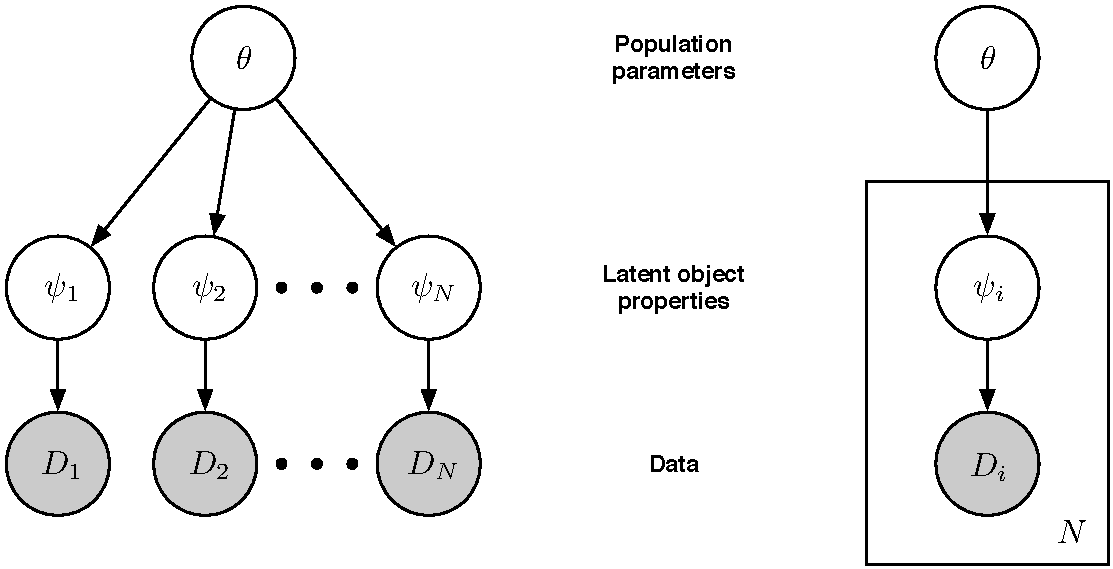
\includegraphics[width=.8\textwidth]{fig/DAG-2Level-Full+Plate}
\end{center}
\caption{Directed acyclic graph (DAG) for a 2-level hierarchical Bayesian model.
\emph{Left}:~DAG explicitly showing replicated conditionally independent subgraphs.
\emph{Right}:~DAG depicting replicated elements with a plate.}
\label{fig:DAG-2Level}
\end{figure}

The DAG describes a generative model for all of the random variables, including the data.
However, when the task is inference of parameters conditional on observed data (versus prediction of unobserved data), specifying member likelihood functions (rather than sampling distributions) can be a significant simplification.
In many astronomical applications, estimation of $\psi_i$ from $D_i$ is often a nontrivial inference problem in itself.
For example, when $\psi_i$ denotes the apparent brightness of a star and $D_i$ denotes image data, inference may involve fitting the complicated point spread function of an imaging instrument to Poisson distributed photon counts in dozens or hundreds of pixels (often marginalizing over an uncertain background or instrument calibration component).
The resulting likelihood function for $\psi_i$ (or marginal likelihood function, when there are nuisance parameters) will often be relatively easy to summarize as a function of $\psi_i$; e.g., it may be well approximated by a Gaussian or multivariate Gaussian function (perhaps after a transformation).
On the other hand, the sampling distribution for the data may be quite complicated and high-dimensional.
In many circumstances, it may not even be well-defined.
Weather or spacecraft conditions may affect the precision, accuracy, and even the quantity of data for a member observation; the repeated sampling distribution may be hard or even impossible to define objectively, while the likelihood function may be well-defined.
Most astronomical surveys produce member estimates with heteroscedastic uncertainties, in the sense of producing member likelihood functions with widths that vary from object to object.
It may be difficult or impossible to accurately describe the repeated sampling properties of the heteroscedastic uncertainties.
But for inference based on \emph{given} observations, only the actually available member likelihood functions matter.
Implementing inference in a manner that requires specifying only the member likelihood functions, rather than the sampling distributions, is a better fit to the nature of astronomical survey catalog data summaries than an implementation requiring unique specification of the lowest level sampling distributions.

A widely-used approach for posterior sampling in the context of two-level hierarchical models is the \textit{Metropolis-within-Gibbs} (MWG) algorithm, where the $\theta$ population parameters and the $\psi_i$ member properties are sampled in separate, alternating steps.
First, the member properties are sampled by holding the population parameters fixed, then the population parameters are sampled by holding the member properties fixed.
These steps may each be implemented with Metropolis or Metropolis-Hastings algorithms; their sequential combination amounts to Gibbs sampling on the joint space.
Explicitly, the steps are:
\begin{align}
\psi_i &\sim p(\psi_i \assm \theta, D_i), \quad\forall i\in 1:N;
\label{eq:psi_sampling} \\
\theta &\sim p(\theta \assm \psivec, M).
\label{eq:theta_sampling}
\end{align}
The departure point for CUDAHM is recognition that, since the $\psi_i$ properties are conditionally independent in \eqref{eq:psi_sampling}, they may be sampled in parallel, making this part of the MWG algorithm suitable for a massively parallel implementation using GPUs.
We describe such an implementation further below.

Since $\psi_i$ may be a vector, the $\psi_i$ node in the DAG may admit a factorization leading to further structure within the plate in Fig.~\ref{fig:DAG-2Level}.
Fig.~\ref{fig:DAGs} shows DAGs for several other single-plate modeling scenarios for which inference may be implemented using MWG with massively parallel sampling of member properties.

\begin{figure}
\begin{center}
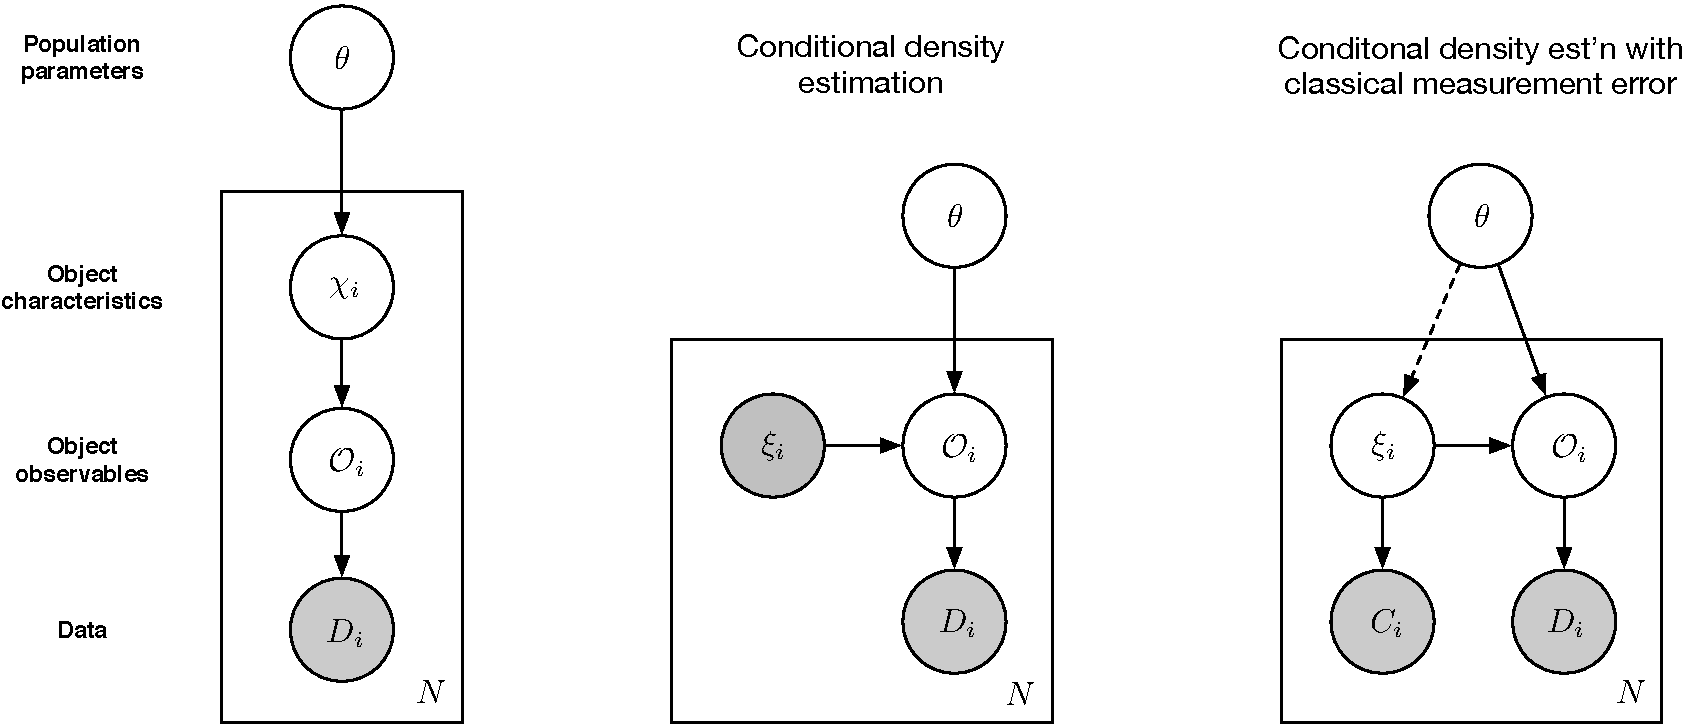
\includegraphics[width=.9\textwidth]{fig/DAGs-3}
\end{center}
\caption{Example single-plate DAGs that may be implemented in CUDAHM.
\emph{Left}: DAG for a 3-level hierarchical model corresponding to demographic inference for objects with latent characteristics $\chi_i$, related to latent observables $\obsv_i$.
\emph{Center}:~DAG for conditional density estimation, expressed via a latent observable $\obsv_i$, and a precisely measured predictor (covariate), $\xi_i$.
\emph{Right}:~DAG for conditional density estimation with classical measurement error, with a latent predictor, $\xi_i$, measured indirectly via data $C_i$.
The predictor may have an a priori known prior distribution, or it may be parameterized (with parameters included in $\theta$, in which case the dashed edge would be present).}
\label{fig:DAGs}
\end{figure}

The DAG in the left panel depicts a frequently arising structure in astronomy, where the object properties $\psi_i$ consist of intrinsic \emph{characteristics} $\chi_i$ that, if known, can predict \emph{observables}, $\obsv_i$, i.e., quantities that can predict observed data.%
\footnote{In astronomical parlance, measurements of the observables are used to ``characterize'' the object, whence our choice of the term ``characteristics'' here.
We reserve the term for properties intrinsic to the source, i.e., not depending on observer-referred quantities such as distance.
E.g., luminosity is a characteristic; flux (brightness at the telescope) is an observable.}
An important example is inference of \emph{number-size distributions} (also known as number counts or $\log N$--$\log S$ distributions).
Here the object characteristics are distance, $r_i$, and luminosity, $L_i$ (amount of energy emitted per unit time).
The observable is flux (rate of energy flow per unit area normal to the line of sight, per unit time, at the telescope), $F_i$, related to the characteristics via the inverse-square law, $F_i = L_i/(4\pi r_i^2)$ (or its cosmological generalization).

The DAG in the middle panel depicts conditional density estimation, where the properties $\psi_i$ are comprised of precisely measurable predictors (covariates), $\xi_i$, that, together with the population parameters $\theta$, specify the PDF for observables, $\obsv_i$; the data provide likelihood functions for the $\obsv_i$.
An important example is inference of a \emph{luminosity function}, which describes the population distribution for the luminosities of a class of sources (say, a stellar or galaxy type).
If the PDF for luminosity is $\lpdf(L;\theta)$, and the distances to objects may be precisely measured (say, via spectroscopic redshift data), then by a simple change of variables the PDF for the flux observable for a source at distance $d$ is $4\pi d^2 \lpdf(4\pi d^2 F; \theta)$ (in Euclidean space).
This would be the distribution for the $\obsv_i$ node in the middle DAG.
We treat a more complicated version of this problem below, where the object sample is subject to flux-dependent selection effects.

As a final example, the DAG in the right panel depicts conditional density estimation with measurement error (i.e., uncertainty in the predictors), with a classical measurement error structure (data distributions conditional on latent predictor values).
A wide variety of astronomical data analysis problems have this structure.
\cite{K+12-DustSEDs} describes a noteworthy example studying how the spectrum of infrared emission from heated interstellar dust depends on properties of the dust grains; this is one of the specific problems motivating CUDAHM.
Earlier studies, based on maximum likelihood estimates of dust properties (ignoring measurement error), found a surprising negative correlation between dust temperature and a spectral index parameter indicating how the dust properties tilt the infrared spectrum away from a black body spectrum.
Accounting for measurement error \emph{reversed the sign} of the inferred correlation, reconciling it with some theoretical models.
\cite{K+12-DustSEDs} analyzed measurements from $\sim 10^4$ dust regions; CUDAHM dramatically accelerates the calculations and makes such studies feasible with 10 to 100 times larger samples.

%-------------------------------------------------------------------------------
\subsection{CUDAHM architecture}
\label{sec:arch}

To sample member propertis in the MWG algorithm, as specified in Eq.~\ref{eq:psi_sampling}, we use the robust adaptive Metropolis (RAM) algorithm devised by \cite{vihola2012robust}.
It works by adaptively refining a Metropolis algorithm proposal distribution during the sampling process until a target mean acceptance rate $\alpha_*$ is reached.
CUDAHM currently uses a multivariate normal distribution as the proposal $q$, and sets the target mean acceptance probability to a default value of $\alpha_{*}=0.4$.
Adaptation involves using new samples to adjust the proposal covariance matrix in a manner that decays with time along the Markov chain so as to guarantee correct asymptotic sampling.
Specifically, adjustments enter with a decaying weight, $\eta_{n}=n^{-2/3}$, where $n$ is the iteration number along the Markov chain.

Following \cite{vihola2012robust}, let $S_{1}$ be the identity matrix and $X_{1}$ some point in the space to be sampled for which the target density $\pi(X_{1})>0$.
Each RAM iteration cycles through the following steps: 
\begin{enumerate} \item Compute $Y_{n}=X_{n-1}+S_{n-1}U_{n}$, where $U_{n}\sim q$ is an independent random vector.
\item With probability $\alpha_{n} \equiv \min\{1,\pi(Y_{n})/\pi(X_{n-1})\}$ the step is accepted, and $X_{n}=Y_{n}$; otherwise the step is rejected and $X_{n}=X_{n-1}$.
\item Compute the lower-diagonal matrix $S_{n}$ with positive diagonal elements satisfying the equation
\begin{equation}
S_{n}S_{n}^{T}=S_{n-1}\left(I+\eta_{n}(\alpha_{n}-\alpha_{*})\frac{U_{n}U_{n}^{T}}{\parallel U_{n}\parallel^{2}}\right)S_{n-1}^{T}
\end{equation}
where $I$ is an identity matrix.
The solution for $S_{n}$ is unique as it is the Cholesky factor of the right hand side.
\end{enumerate}
CUDAHM implements these steps on the GPU, via ``kernel'' code (code executed on a GPU) written in the CUDA language and taking advantage of optimized CUDA library functions (e.g., for random number generation and linear algebra).
The population sampling step in the MWG algorithm, as specified in Eq.~\ref{eq:theta_sampling}, is executed on the host CPU, using code written in standard \Cpp.
\enote{Are some parts of this step done on the GPU?}

%\enote{Provide some further details about the CUDAHM architecture, e.g., how users must structure their code, classes/structures available for passing information to/from the GPU, how random number generation is handled, etc..}

\enote{New text from Janos below; this needs some massaging; we also need to provide a link to the main CUDAHM repo here:}

CUDAHM enables one to easily and rapidly construct an MCMC sampler for a simple hierarchical model, requiring the user to supply only a minimimal amount of CUDA code. 
%CUDAHM assumes that a set of observed data $\{D_i\}$ are available for a sample of objects, and that these measurements are related to an unobserved set of member properties. This framework can simultaneously sample the values of these properties and the population parameters in two steps as it is mentioned earlier. The first step (2.4) is done in parallel for each object on the GPU, while the proposals for second step (2.5) are generated on the CPU, but the calculations are performed on the GPU.
There are four main classes in CUDAHM that users may need to use directly:
\begin{itemize}
\item \texttt{DataAugmentation}: This class controls the calculations involving the member properties.
\item \texttt{PopulationPar}: This class controls the calculations involving the population parameters.
\item \texttt{GibbsSampler}: This class runs the MWG sampler.
\item \texttt{GibbsSamplerWithCompactMemoryUsage}: This class also runs a MWG sampler, but with more efficient use of memory. It opens an output file stream (which has a buffer) and writes samples out on the fly.
\end{itemize}

The simplest use case involves only instantiating the \texttt{GibbsSampler} class, since this will internally construct \texttt{DataAugmentation} and \texttt{PopulationPar} objects, using reasonable default algorithms.
However, if one wants to subclass the \texttt{DataAugmentation} or \texttt{PopulationPar} classes, to customize algorithms to the problem, or to generalize the framework, then pointers to the instances of these classes must be provided to the \texttt{GibbsSampler} constructor.
In general this is only needed if one wants to override the default methods for setting the initial values, or if one wants to override the default prior on the population parameters (which is an uninformative uniform distribution).

We note the CUDAHM default methods assume \emph{all} member properties are uncertain; kernel functions that are used for updating member properties and the population parameters on the GPU assume all member properties may change in each MWG cycle.
This is important to consider for problems where the object properties contain precisely measurable predictors (e.g., covariates for conditional density estimation in the manner of the middle DAG in Fig.~\ref{fig:DAGs}), which should be held fixed over the course of posterior simulation.
When this is the case, the user should override the default methods.
The \texttt{lum\_func} implementation, which is related to the luminosity function example case, provides concrete guidance on this issue.
We are exploring internal architectural changes to simplify the user API for handling such cases.

There are two functions that the user must provide: a function that computes the logarithm of the probability density of the measurements given the member properties for each object in the sample, and a function that computes the logarithm of the probability density of the member properties given the parent population parameters.
These functions execute on the GPU and must be written in CUDA.
The file \texttt{cudahm\_blueprint.cu} under the \texttt{cudahm} directory contains a blueprint with documentation that the user may use when constructing their own MCMC sampler.


%===============================================================================
%\section{Example: Dust properties in a star-forming region}
%\label{sec:dust}
%
%\enote{Add material here for Brandon's dust SED example if desired; we should probably try to save this for the A\&C version.}
%===============================================================================

% These perhaps should be merged:
%===============================================================================
\section{Luminosity function estimation: Framework}
\label{sec:lum_func}

The CUDAHM distribution contains some example code implementing basic hierarchical models, such as the normal-normal model, and a realistically complicated astrophysical example handling regression with classical measurement error, with nonlinear models (the interstellar dust problem described above).

As a somewhat more complicated application of CUDAHM, we here consider luminosity function estimation, a parametric conditional density estimation problem arising across many areas of astronomy.
We highlight this example, both because of its ubiquity across astronomy, and to illustrate the generality of CUDAHM.
We describe luminosity function estimation for a model including not only measurement error, but also \emph{selection effects}.
The selection effects make the joint distribution structure more complicated than the conditional density estimation DAG shown in Fig.~\ref{fig:DAGs}; in particular, there are two plates (corresponding to detected and undetected objects).
However, the likelihood function can be manipulated to have a conditional dependence structure similar to that of a single-plate DAG, allowing straightforward implementation of the model using CUDAHM.

%-------------------------------------------------------------------------------
\subsection{Astronomical background}
\label{sec:LF-astro}

%\enote{Introductory content here was moved from Janos's intro.}

The fundamental observables for localized astronomical sources include position (both direction on the celestial sphere, and distance, $r$, in some chosen coordinate system), and apparent brightness, quantified in terms of flux, $F$ (energy or photon number per unit time per unit area normal to the line of sight).
Astronomers use these observables to study demographic properties of many classes of sources, including stars and galaxies of various types, minor planets (such as asteroids), and explosive transients (gamma-ray bursts, supernovae).
For concreteness, here we focus on observations of nearby galaxies, for which distance may be measured by using spectroscopy to find the \emph{redshift}, $z$, of spectral lines (i.e., their fractional shift in wavelength from laboratory values).
Due to the cosmological expansion, for relatively nearby galaxies outside the local group, distance is proportional to redshift to a good approximation, with
\begin{equation}
r = \frac{cz}{H_0},
\label{eq:H0}
\end{equation}
where $c$ denotes the speed of light, and $H_0$ is Hubble's constant, measuring the current expansion rate of the universe, with $H_0 \approx 70$~km~s$^{-1}$~Mpc$^{-1}$ (with Mpc denoting megaparsecs).
$H_0$ is measured with a precision of several percent, and spectroscopic redshifts for nearby galaxies can be measured to sub-percent precision.
For simplicity, here we consider distances to be precisely measured, via spectroscopic redshifts.
Often, astronomers use redshift directly as a proxy for distance.

A fundamental intrinsic characteristic of a source is its \emph{luminosity} (emitted power), $L$, a measure of its intrinsic (vs.\ apparent) brightness (with units of energy per unit time).
For nearby galaxies (i.e., for distances where space is very nearly Euclidean), the inverse-square law relates $L$ to the observables $F$ and $r$:
\begin{equation}
F=\frac{L}{4\pi r^2}.
\label{eq:inv-sqr}
\end{equation}
The \emph{luminosity function}, $\lfunc(L, r)$, describes the distribution of luminosities for a population at a specified distance (or redshift).
It is typically defined as the intensity function for a point process, i.e., as specifying the expected number of galaxies per unit volume at distance $r$, per unit luminosity interval.
If we denote the spatial number density of galaxies at distance $r$ by $n(r)$, then $n(r) = \int dL\, \lfunc(L, r)$.
The \emph{luminosity PDF} for galaxies at distance $r$ is then
\begin{equation}
\lpdf(L,r) = \frac{\lfunc(L, r)}{n(r)}.
\label{eq:lpdf}
\end{equation}
Note that $\lfunc(L,r)$ and $\lpdf(L,r)$ specify \emph{conditional} distributions, i.e., distributions for $L$ at a given $r$.%
\footnote{Authors vary on the definition of the luminosity function, many defining it as done here, and others using ``luminosity function'' to denote what we here call the luminosity PDF.}
Using (\ref{eq:inv-sqr}), the \emph{flux PDF} for galaxies at distance $r$, denoted $\rho(F,r)$, can be found by a change of variables from $L$ to $F$, giving
\begin{equation}\label{eq:fluxPDF}
\rho(F,r) = 4\pi r^2 f(4\pi r^2 F, r).
\end{equation}

The galaxy luminosity function carries valuable information about the formation and evolution of galaxies, therefore it is an important target of inquiry in astronomy (see \citealt{BST88-LumFuncReview} and \citealt{J11-LumFuncReview} for reviews).
\citealt{J11-LumFuncReview} provides a review of methods developed by astronomers for estimation of galaxy luminosity functions.
CUDAHM can address parametric luminosity function inference; this section provides an example as a demonstration of CUDAHM's capability and flexibility.
In the next subsection, we describe a useful parametric family of luminosity functions.
Then we present a hierarchical Bayesian framework for modeling astronomical survey data using thinned latent marked point process models, developing it specifically for luminosity function inference.
The next section presents a simulation study demonstrating CUDAHM luminosity function inference for simulated populations with sizes up to $10^6$.

% For simplicity we here focus on a homogeneous population, so that $n(r)$ is considered fixed (constant with respect to volume measure).
% The following development is straightforward to generalize to account for models with distance dependence in the luminosity function.

%-------------------------------------------------------------------------------
\subsection{Parametric luminosity function models}
\label{sec:lfmodels}

For most cosmic populations, including galaxies, the luminosity function falls very steeply with increasing luminosity.
The canonical starting point for parametric modeling of luminosity distributions is the \emph{Schecter function},
\begin{equation}
\lfunc(L;\theta) =
  \frac{A}{L_*} \left(\frac{L}{L_*}\right)^{\beta} e^{-L/L_*},
\label{eq:schecter}
\end{equation}
where the parameters $\theta = (L_*,\beta, A)$ comprise a luminosity scale, $L_*$, a power law index, $\beta$, and an amplitude, $A$.%
\footnote{There are varying conventions for parameterizing the amplitude of the Schecter function.
In this parameterization, $A$ has units of space density.
In similar parameterizations, $A$ is often denoted $\lfunc_*$, although it neither has the units of $\lfunc$, nor is it equal to $\lfunc(L_*)$, as the symbol might misleadingly suggest.}
The form of the Schecter function would seem to imply a luminosity distribution that is a gamma distribution (with shape parameter $\alpha = \beta - 1$).
However, the observed samples of many populations follow Eq.~\ref{eq:schecter} with $\beta$ in the interval $(-2,-1)$, in which case the integral of $\lfunc(L;\theta)$ over $L$ is infinite, and the luminosity distribution is formally improper (with $\alpha$ outside of the allowed range for the gamma distribution).
Low-luminosity sources are unobservable (due to noise and background, discussed below), so in practice the \emph{observable} luminosity function is truncated at low luminosities, and the impropriety is often ignored.
But the actual luminosity function must rise less quickly with decreasing $L$ (corresponding to $\beta$ becoming larger than $-1$) or be cut off at low luminosities (corresponding to there being a minimum galaxy size).

%\enote{Perhaps move some of the following details to an appendix?}

For some populations, an increase in the power law index (i.e., flattening of the logarithmic slope) is in fact observed at low luminosities.
This has been observed for quasars (galaxies with a large, actively accreting central black hole; see \citealt{M+13-QuasarLumFunc}).
Similarly, the stellar initial mass function (related to the stellar luminosity function, and fit with similar models) has a low-mass (low-luminosity) index that flattens by $\approx 1$ (\citealt{K07-IMF-BPL}).
Motivated by such observations, and to keep the luminosity distribution proper, we here adopt a ``break-by-one'' (BB1) generalization of the Schecter function, with $\lfunc \propto L^{\beta+1}$ at low luminosities, and thus integrable for $\beta > -2$.
Specifically, the BB1 model has a luminosity distribution with three parameters: a mid-luminosity power law index, $\beta$, and two parameters defining the mid-luminosity range, $(l, u)$, with $l < u$ and  $u$ playing the role of $L_*$ in the Schecter function, and the power law index smoothly breaking to $\beta+1$ as $L$ decreases below $l$.
The BB1 luminosity PDF has following functional form:
\begin{equation}
\label{eq:lumPDF} 
\lpdf(L ; \theta) = 
  \frac{C(\beta,u,l)}{u}\left(1-e^{-L/l}\right) \left(\frac{L}{u}\right)^{\beta} e^{-L/u},
\end{equation}
where the normalization constant $C(\theta)$ is
\begin{equation}
\label{eq:normLumPDF} 
C(\beta,u,l) =
  \begin{cases} \dfrac{1}{\Gamma(\beta+1)\cdot\left(1-\frac{1}{\left(1+\frac{u}{l}\right)^{\beta+1}}\right)} 
    & \quad \text{if } \beta > -2\text{ and }\beta \ne -1; \\
 \dfrac{1}{\log\left(1+\frac{u}{l}\right)} & \quad \text{if } \beta=-1.
  \end{cases}
\end{equation} 
Note that as $l\rightarrow 0$, the BB1 distribution becomes a gamma distribution (if $\beta > -1$).
%Also, in our computational implementation, the condition $\beta=-1$ of the first case is $-1.001<\beta<-0.999$.
We designed the BB1 distribution to have smooth power law break behavior at low $L$, yet also have an analytical normalization constant;
it is proper for $\beta > -2$.
It can also be sampled from using a straightforward modification of a widely-used algorithm for sampling from the gamma distribution (\citealt{ahrens_computer_1974}).
These properties make it useful for simulation experiments.

We define a BB1 luminosity function by multiplying the BB1 luminosity distribution by the galaxy spatial number density, which is simply a constant, $n$, for a homogeneous population.
Fig.~\ref{fig:lumfunc} shows an example BB1 luminosity function, with $\beta = 1.5$, and $(l,u) = (5\times 10^{10}, 5\times 10^{12})$ in dimensionless units; it is plotted both with $\log$-linear axes, and with $\log$-$\log$ axes, where the varying power law behavior is evident.
The local power law index corresponds to the slope, $G(L)$, in $\log$-$\log$ space, defined by
\begin{equation}
	G(L) \equiv \frac{\dd\log{\lpdf}}{\dd\log{L}} = \frac{L}{\lpdf} \frac{\dd \lpdf}{\dd L} = g(L) + \beta - \frac{L}{u},
\end{equation}
with
\begin{equation}
	g(L) = \frac{L}{l}\cdot\frac{1}{e^{L/l} - 1}.
\end{equation}
Evidently, $g(L) \rightarrow 0$ for $L \gg l$ and $g(L) \rightarrow 1$ for $L \ll l$.
Thus the logarithmic slope, $G(L)$, corresponds to an exponential cutoff at large $L$, and at small $L$, a slope of $\beta + 1$.
When $u\gg l$, so there is a range where $L\gg l$ but $L\ll u$, the logarithmic slope is $\approx \beta$ in that range.

\begin{figure}
	\begin{subfigure}[c]{0.45\textwidth}
		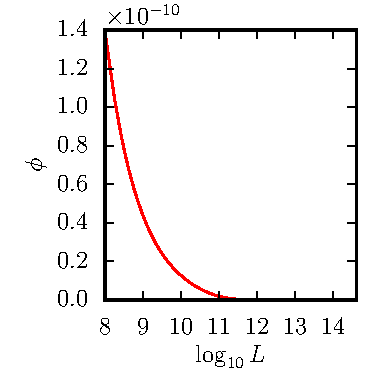
\includegraphics{fig/lumfunc_loglin}
		\caption{}
	\end{subfigure}
	\begin{subfigure}[c]{0.45\textwidth}
		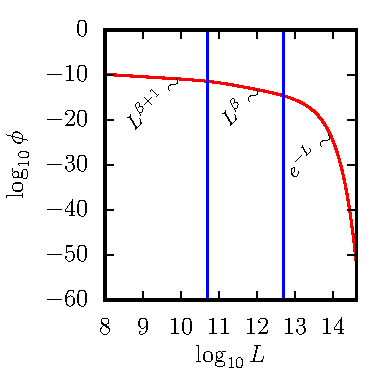
\includegraphics{fig/lumfunc_loglog}
		\caption{}
	\end{subfigure}
	\caption{Example BB1 truncated broken power law PDF, on a log-linear scale (a) and on log-log scale (b), with parameters $(u,l) = (5\times 10^{10}, 5\times 10^{12})$ in dimensionless units, and $\beta = -1.5$.
	In Panel~b the blue verticals show the lower limit $l$ and upper limit $u$ of the region where the power law slope is $\approx\beta$.}
	\label{fig:lumfunc}
\end{figure}

Finally, the BB1 cumulative distribution function is 
\begin{equation}
\label{eq:lumCDF} 
\lcdf(L ; \theta) = 
  C(\theta)
  \left[ \Gamma(\beta + 1) - \gamma\left(\beta + 1, L/u\right) - \frac{\Gamma(\beta + 1)-\gamma\left(\beta + 1, L\cdot\left(\frac{1}{u}+\frac{1}{l}\right)\right)}{\left(1 + \frac{u}{l}\right)^{\beta + 1}} \right],
\end{equation}
where $\Gamma(\cdot)$ and $\gamma(\cdot, \cdot)$ denote the gamma function and the upper incomplete gamma function, respectively.

%-------------------------------------------------------------------------------
\subsection{Modeling survey selection effects and measurement error}
\label{sec:slxn+err}

Astronomers estimate luminosity functions and other astronomical distributions using data compiled in \emph{survey catalogs}: tables of estimates (including uncertainties) of object properties, accompanied by a description of selection criteria for the survey that produced the catalog.
Catalogs are derived data products; they summarize information in more complex and voluminous raw datasets, such as large collections of images or time series.
The nature of astronomical catalog data makes their analysis differ in some respects from analyses of survey data familiar in the statistical survey sampling literature.

Flux measurements are affected by measurement error that is often dominated by Poisson fluctuations in the photon counting rate, including fluctuations from astrophysical and instrumental backgrounds.
The measurement error thus approximately scales with the square root of the flux, and is fractionally greater at low flux than at high flux.
At low fluxes, photons from the backgrounds can produce false source detections.
To prevent this, surveys adopt detection criteria to strongly mitigate against false detections.
A simple, representative criterion is to accept sources only if the estimated flux is $\nu$ times the flux uncertainty, with $\nu \approx 5$ so that the probability for false detection is low even for large catalogs (i.e., there is strong control of the family-wise error rate).

Detection criteria introduce \emph{selection effects} into catalogs.
Most obviously, faint sources (low luminosity sources, or distant high luminosity sources) are excluded; the observable luminosity function is a thinned version of the actual luminosity function.
In addition, \emph{measurement error} more subtly but significantly distorts the shape of the observable distribution, a phenomenon well known in the density deconvolution literature, and also recognized in the astronomical literature, where it is sometimes called \emph{Eddington bias}, in reference to early discussions of the distortion by Eddington and Jeffreys (REFS).
They noted that an object with a measured flux of $\hat F$ is more likely to be an object with a true flux $F < \hat F$ than one with $F > \hat F$, even when measurement errors have a symmetric distribution, because dim sources are more numerous than bright sources in most astronomical settings.
Selection effects can exacerbate the distortion in the vicinity of a flux threshold, with measurement error and the falling flux distribution conspiring to scatter more below-threshold sources into the observed sample than above-threshold sources out of it, a component of what astronomers call \emph{Malmquist bias} \citep{binney1998galactic} (although the term is used inconsistently).
Hierarchical modeling can automatically account for such thinning and distortion, in a manner that adapts to the shape of the luminosity function; this is a major motivation for its increasing popularity in astrostatistics.

We have developed a framework for modeling astronomical survey data using \emph{thinned latent marked point process models}.
Measurement error is handled in a hierarchical Bayesian manner, by introducing latent member property parameters, with catalog estimates understood as describing member likelihood functions for the properties.
We model the population distribution of the latent member properties using marked point processes.
We model selection effects through thinning of the latent point process.
This framework was originally developed for studying the luminosity function of gamma-ray bursts, powerful explosive transients thought to mark the birth of stellar-mass black holes (\citealt{LW95-GRBs-TLPP,LW98-GRBs-Iso}).
It was subsequently adapted to study the luminosity distribution (and through it, the size distribution) of trans-Neptunian objects, asteroid-like minor planets in the outer solar system (\citealt{L04-MsmtErr,P+08-TNOSizeDistn}).
We outline the framework here as it applies to luminosity function estimation and similar problems, in contexts where a marked Poisson point process is an appropriate model for the latent member properties.
\cite{kelly2008flexible} independently developed a similar approach for settings where a binomial point process may be appropriate, and applied it to estimating the number density of quasars as a function of redshift.

A somewhat subtle aspect of the problem is the tie between measurement error and selection effects.
In astronomical surveys, the raw data are searched to find candidate objects.
For candidates that pass detection criteria, the data are used to estimate source properties.
The same underlying data are used both for selection (detection) and measurement; these tasks are not independent, as is assumed in many statistical survey methods outside of astronomy.
Ignoring the dependence can corrupt inferences.

Object detection is typically implemented via a scanning procedure.
For example, for image data, a fixed aperture may be scanned over the image; a detection algorithm determines if an object is present, e.g., by comparing the estimated flux in the aperture to a threshold value (set by background and noise estimates), or by fitting an image model to the data in the aperture and comparing the fitted amplitude to a threshold.
For time series data, a window may be scanned over the time series, with an object detected if the estimated flux is above a threshold.
If an object is detected, its properties are estimated, e.g., by a likelihood or weighted least squares calculation, with estimation results summarized in the catalog.

Fig.~\ref{fig:ScanMark} illustrates the framework and its relationship to catalog construction.
We split the object property parameter space into scan and mark components.
The scan component corresponds to the dimensions over which the detection scan operates; 
%(e.g., two-dimensional position for image data, or arrival time for time series data).
the mark component corresponds to the remaining dimensions.
For our galaxy luminosity function example, the scan component is the two-dimensional position of the galaxy image on the detector (corresponding to its direction on the sky), and the mark component is the galaxy luminosity and distance, or equivalently, flux and distance (in a more complex case, the mark component might include color and morphological parameters).
In the figure, the dots (red) indicate the true properties of seven galaxies; the blue contours depict likelihood functions for the properties, based on noisy image data.
The gray region at the bottom is bounded above by the position-dependent detection threshold; an object is detected only if its best-fit (maximum likelihood) flux is above the threshold.
Here two of the seven galaxies are not detected.

\begin{figure}
\begin{center}
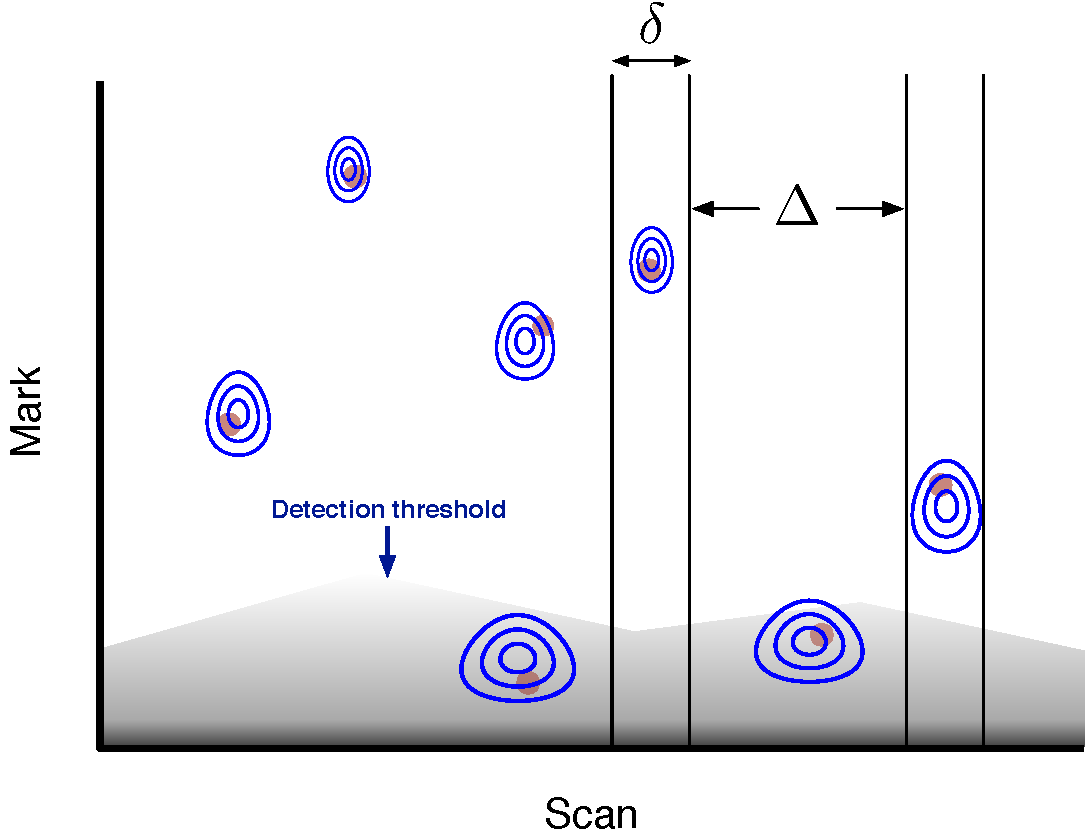
\includegraphics[width=.8\textwidth]{fig/ScanMarkPtProcess-Thin+Err}
\end{center}
\caption{Depiction of thinned latent marked point process model for catalog data produced by an astronomical survey.
Object properties are split into a scanned subset and a mark subset.
Dots (red) show latent (true) values for an object's properties.
Contours (blue) depict member likelihood functions from analysis of the raw survey data; catalogs provide summaries of these for detected objects.
Gray region at bottom depicts the non-detection region; candidates with estimated mark values below a varying threshold are rejected.
$\delta$ and $\Delta$ denote sizes of detection and nondetection intervals.}
\label{fig:ScanMark}
\end{figure}

We model the properties using a (latent) marked Poisson point process, i.e., a Poisson point process for the scanned parameters, and a probability density function for the mark parameters.
For concreteness, we focus on the luminosity function example, taking the scan parameter to be object position, $x$ (a 2-vector), and the mark parameters to be flux and distance, $(F, r)$.
We suppose that the spatial density of galaxies is approximately constant over the region probed by the survey.
There is thus a constant Poisson intensity parameter, $\lambda$, describing the distribution of galaxies in $x$.
We assume a BB1 luminosity PDF, independent of distance (of course, the flux PDF will depend on distance, thanks to the inverse square law).
The flux and distance mark PDF is thus a product of PDFs, $h(r)\rho(F,r)$.
For $\rho(F,r)$ we adopt the BB1 luminosity PDF form of (\ref{eq:lumPDF}), with parameters $\rhopar = (\beta,u,l)$, related to $\rho(F,r)$ via (\ref{eq:fluxPDF}); we write the flux PDF as $\rho(F,r; \rhopar)$ when we want to display the parameter dependence.
For the PDF for galaxy distance, $h(r)$, the assumption of homogeneity implies
\begin{equation}\label{eq:distPDF}
h(r) = 
\begin{cases} 
    \dfrac{3r^{2}}{r_u^{3}} & \quad \text{if } 0\leq r\leq r_u,\\
    0 & \quad \text{otherwise},
\end{cases} 
\end{equation}
where $r_u$ is an upper limit on distance chosen to be beyond the surveyed volume.%
\footnote{That is, chosen so that the most luminous galaxies of interest (i.e, with $L$ of order $u$ in the BB1 model) have fluxes comfortably below the lowest flux threshold.
In deep surveys (reaching to very dim fluxes), cosmological considerations, including the finite age of the universe and the non-Euclidean geometry of spacetime, ameliorate the growth of $h(r)$ with $r$.}
The population model thus has parameters $\ppar = (\lambda,\rhopar)$.

We consider a case where we have precise distance measurements for the galaxies (e.g., from high-resolution spectroscopic data providing precise redshifts).
We assume independent errors in the position and flux measurements, so the catalog contains descriptions of separate member likelihood functions for flux and position, denoted $\ell_i(F)$ and $m_i(x)$ for galaxy $i$, with $i=1$ to $N$.
Formally, denoting the image data for detected galaxy $i$ by $D_i$, we are writing
\begin{equation}\label{eq:xFr-like}
p(D_i|x,F,r) = \ell_i(F)\, m_i(x)\, \delta(r - r_i),
\end{equation}
where the Dirac delta function factor represents the precise measurement of distance.
We must also describe the survey's selection effects.
These are determined by the detection threshold as a function of the scan location.
At each scanned location, $x$, the threshold determines the set, $\dtxns_x$, of possible data (i.e., images) that would be deemed detections.
For example, if the detection criterion is that the MLE flux estimate, $\hat F(D)$ for data $D$, must exceed a threshold $\Fth(x)$, then $\dtxns_x = \{D : \hat{F}(D) > \Fth(x)\}$.
Reporting $\dtxns_x$, or equivalently $\Fth(x)$, then describes the selection effects.
But we will see below that a simpler summary of the detection criteria will suffice.


We now compute the likelihood function for the parameters, based on catalog data describing member likelihood functions and the selection effects.
The construction we use is illustrated in Fig.~\ref{fig:ScanMark}.
We partition the scan space into $N$ detection intervals, $\delta_i$, containing a single detected object, and $M$ nondetection intervals, $\Delta_j$, in which no candidate object passed the detection criterion.%
\footnote{We are presuming that galaxy images are well-separated, i.e., we do not treat here the \emph{crowded field} case, where the images of distinct objects may strongly overlap.}
The likelihood function is the product of the (conditionally independent) probabilities for these intervals.

We first consider the probability for no detection in one of the $\Delta_j$ intervals.
We break it up into subintervals of size $\delta x$, small enough that the detection threshold is approximately constant over the interval.
The probability for seeing no detections in $\delta x$ is the sum of the probabilities for the following events (conditioned on the population parameters, $(\lambda,\rhopar)$):
\begin{itemize}
\item No objects have $x$ in the interval.
\item One object has $x$ in the interval, but it produced data that were not in $\dtxns_x$.
\item Two objects have $x$ in the interval, but both produced data that were not in $\dtxns_x$.
\item And so on\ldots.
\end{itemize}
Each event is a conjunction of two simpler events, the Poisson probability for the specified number of objects lying in the interval, and the probability for not detecting any events in the interval.
We will express the latter probability in terms of the \emph{detection efficiency} at $x$ for objects with flux $F$,
\begin{align}\label{eq:eta-def}
\effic(x,F) 
  &= p(D\in\dtxns_x | F)\\
  &= p(\hat{F}(D) > \Fth(x) | F),
\end{align}
where the condition $F$ denotes that an object is present with flux $F$.
The probability for detecting an object with a given location and distance but unspecified flux and distance, given the population parameters, is then
\begin{equation}\label{eq:p-x}
p_x(\rhopar) = \int dr \int dF\,\rho(F,r)\, h(r)\, \effic(x,F).
\end{equation}
The probability for \emph{not} detecting an object with a given location is then $1-p_x(\rhopar)$.

Now let $\nu$ denote the (unknown) number of objects with $x$ in $\delta x$.
Then the probability for no detections in $\delta x$ at $x$ is
\begin{align}\label{eq:q-exp}
q(x) 
  &= \sum_{\nu=0}^\infty \frac{(\lambda\delta x)^\nu}{\nu!} e^{-\lambda\delta x}
        \left[1 - p_x(\rhopar)\right]^\nu\nonumber\\
  &= e^{-\lambda\delta x} \sum_{\nu=0}^\infty \frac{(\lambda\delta x)^\nu \left[1 - p_x(\rhopar)\right]^\nu}{\nu!}
          \nonumber\\
  &= \exp\left[-\lambda\delta x p_x(\rhopar)\right].
\end{align}
This is the probability for no detections in a subinterval of a $\Delta_j$ interval.
The probability for no detections across the entire interval is the product of its subinterval probabilities.
The exponents add, so that the nondetection probability becomes
\begin{equation}\label{eq:q-def}
q(\Delta_j) = \exp\left[-\lambda\int_{\Delta_j}dx \int dr \int dF\,\effic(x,F)\, h(r)\, \rho(F,r)\right].
\end{equation}
This is just the Poisson probability for seeing no events, when the expected number of events is $\lambda$ times the fraction of the population expected to be detected in the interval, given the threshold behavior (encoded in the detection efficiency).

Now consider the probability for the data associated with a detection interval, $\delta_i$; for simplicity, we assume all of these intervals are of the same size, $\delta$, in $x$.
The probability for getting data $D_i$ from detection of an object in $\delta_i$ is the sum of the probabilities for the following events:
\begin{itemize}
\item One object has $x$ in the interval, and was detected producing data $D_i$.
\item Two objects have $x$ in the interval, one of which was detected producing $D_i$, with the other undetected.
\item And so on\ldots.
\end{itemize}
To simplify the calculation, let us stipulate that the detected object has values of $(x,F,r)$ in small intervals $(dx, dF, dr)$; at the end, we will account for their uncertainty via marginalization.

The first case is simple; the probability for one object in the interval, having the specified properties, and being detected producing $D_i$, is
\begin{equation}\label{eq:dtxn1}
p_1(\lambda,\rhopar) = 
  (\lambda \delta) e^{-\lambda \delta} 
  \left[\frac{dx}{\delta}\, h(r)dr\, \rho(F,r;\rhopar)dF\right]
  p(D_i\in\dtxns_x, D_i|x,F,r).
\end{equation}
The final probability is for a conjunction; it may be written
\begin{equation}\label{eq:dtxn-joint}
p(D_i\in\dtxns_x, D_i|x,F,r) = p(D_i|x,F,r)\, p(D_i\in\dtxns_x | D_i),
\end{equation}
where we have dropped $(x,F,r)$ from the last factor because the values of the properties are irrelevant for determining detection, once the data are in hand.
Now note that detection is deterministic given the data, i.e., either the data correspond to a candidate meeting the detection criteria or not.
But for a detected object, by definition the data met the criteria, so the last factor is equal to unity.
The first factor we recognize as the member likelihood function, defined in (\ref{eq:xFr-like}).
%\begin{equation}\label{eq:ell-m}
%p(D_i|x,F,r) = \ell_i(F)\, m_i(x)\, \delta(r - r_i).
%\end{equation}
This completes the computation of $p_1(\lambda,\rhopar)$.

For cases with $\nu > 1$ objects present, we will have a factor like $p_1(\lambda,\rhopar)$ for the detected object, and nondection probabilities like the $[1 - p_x(\rhopar)]$ factor appearing in the $\Delta_j$ probability derived above.
But in addition, we have to account for not knowing which of the $\nu$ objects is detected.
The resulting probability for the case of $\nu$ objects present can be written as follows:
\begin{equation}\label{eq:dtxn-nu}
\begin{split}
p_\nu
  &= \frac{(\lambda\delta)^\nu}{\nu!}  e^{-\lambda\delta}\\
  &\quad \times \left(\frac{dx}{\delta}\, h(r)dr\, \rho(F,r;\rhopar)dF\right) \ell_i(F)\, m_i(x)\, \delta(r - r_i) \\
  &\quad \times \left[1 - p_x(\rhopar)\right]^{\nu-1}\\
  &\quad \times \nu.
\end{split}
\end{equation}
Line by line, the factors are:
\begin{itemize}
\item the Poisson probability for $\nu$ objects being in the interval,
\item the probability for one of them having the given properties and
producing the detection data, $D_i$,
\item the probability for the remaining objects not being detected,
\item a factor of $\nu$ from summing over the possibilities for
which of the $\nu$ objects is detected.
\end{itemize}
To facilitate summing the $p_\nu$ probabilities over $\nu$, we gather the $\nu$-dependent terms in (\ref{eq:dtxn-nu}) as follows:
\begin{equation}\label{eq:dtxn-nu2}
\begin{split}
p_\nu
  &= (\lambda\delta)\,  e^{-\lambda\delta}
  \left(\frac{dx}{\delta}\, h(r)dr\, \rho(F,r;\rhopar)dF\right) \ell_i(F)\, m_i(x)\, \delta(r - r_i) \\
  &\quad \times \frac{1}{(\nu-1)!}(\lambda\delta)^{\nu-1}
    \left[1 - p_x(\rhopar)\right]^{\nu-1}.
\end{split}
\end{equation}
Upon summing over $\nu \ge 1$, and marginalizing over the uncertain values of $(x,F,r)$, we find that the probability for the detection data in interval $\delta_i$ is
\begin{equation}\label{eq:p-dtxn}
p(D_i|\lambda,\rhopar) =
  q(\delta_i)\, h(r_i)\, (\lambda\delta)\,
  \left[\int_{\delta_i}\frac{dx}{\delta}\, m_i(x)\right]
  \left[\int dF\, \rho(F,r_i;\rhopar)\, \ell_i(F)\right],
\end{equation}
where $q(\delta_i)$ is an exponential of an integral of the same form as in the nondetection probability in (\ref{eq:q-def}).

The likelihood function is the product of detection probabilities (\ref{eq:p-dtxn}) and nondetection probabilities (\ref{eq:q-def}) for all of the $\delta_i$ and $\Delta_j$ intervals.
All of these probabilities share an exponential factor resembling (\ref{eq:q-def}).
In the product, there will be a sum of the integrals in the exponents; this corresponds to a single integral over the entire $x$ domain of the survey, of the form:
\begin{equation}\label{eq:int3}
\lambda\int_\Omega dx \int dr \int dF\,\effic(x,F)\, h(r)\, \rho(F,r;\rhopar),
\end{equation}
where $\Omega$ denotes the full range of positions surveyed (which would be measured in terms of solid angle on the sky).
Note that the only $x$-dependent factor in the integrand is the detection efficiency.
This lets us write the integral in simpler manner.
Introduce the \emph{average detection efficiency},
\begin{equation}\label{eq:aeffic}
\aeffic(F) \equiv \frac{1}{\Omega} \int_\Omega dx \,\effic(x,F).
\end{equation}
Using this, (\ref{eq:int3}) can be written as a two-dimensional integral,
\begin{equation}\label{eq:int-aeffic}
(\lambda \Omega) \int dr \int dF\,\aeffic(F)\, h(r)\, \rho(F,r;\rhopar).
\end{equation}
The factor $(\lambda \Omega)$ is the expected number of objects in the surveyed region, which depends only on the $\lambda$ parameter.
The remaining factor is the fraction of these that are detectable; it depends only on the remaining population parameters, $\rhopar$.

Equation (\ref{eq:int-aeffic}) shows that the average efficiency is a kind of sufficient statistic for the survey's threshold behavior.
Although catalog builders must determine the detection efficiency over the entire range of the survey, they need only report the lower-dimensional average efficiency for analysts.

We can now write down the full likelihood function for the luminosity function parameters.
Dropping some factors that do not depend on the parameters, the likelihood function is
\begin{equation}\label{eq:like}
\begin{split}
\like(\lambda, \rhopar)
  &= \lambda^N \exp\left[- (\lambda \Omega) \int dr \int dF\,
            \aeffic(F)\, h(r)\, \rho(F,r;\rhopar)\right]\\
  &\quad\times \prod_{i=1}^N h(r_i) \int dF\, \rho(F,r_i;\rhopar)\, \ell_i(F).
\end{split}
\end{equation}
This likelihood function is reminiscent of that for an inhomogenous Poisson point process, whose likelihood is proportional to a product of intensity function factors, evaluated at the observed points, and an exponential whose negative argument is the integral of the intensity function over the observed domain.
One difference is the integral over the latent observable, $F$, in the product factor; this accounts for measurement error.
A more subtle difference is that integrand in the exponential is not the same function playing the role of the intensity function in the product factor.
There is an average efficiency factor in the exponential, but not in the product factor.
This is because of a feature of astronomical surveys noted earlier: the data used for characterization (estimating latent parameters) is also used for detection.
As a result, were one to insert an efficiency factor into the product terms, the data would be doubly used.
This appeared explicitly in our derivation; the text after (\ref{eq:dtxn-joint}).
Some heuristic derivations of similar likelihood functions in the astronomical literature have missed this point, instead inserting an $\aeffic(F)$ factor in the detected object integrals in the likelihood function.
This corrupts inferences; see \cite{L04-MsmtErr} for further discussion.

Notably, the Poisson process intensity parameter, $\lambda$, appears in the likelihood function only as the power, $\lambda^N$, and multiplying the integral in the exponential.
As a result, if we adopt a conjugate prior for $\lambda$ (a gamma distribution), we can easily compute the marginal likelihood function for the $\rhopar$ parameters.
For simplicity, we adopt the limiting case of a uniform prior for $\lambda$.
Marginalizing over $\lambda$ and dropping some $\rhopar$-independent terms, we find that the marginal likelihood function for $\rhopar$ takes the form
\begin{equation}\label{eq:mlike}
\like_m(\rhopar)
  = \prod_{i=1}^N \int dF\, \epdf(F,r_i;\rhopar)\, \ell_i(F),
\end{equation}
where we have introduced an \emph{effective density} for the latent observables, $F$ and $r$,
\begin{equation}\label{eq:epdf}
\epdf(F,r;\rhopar) \equiv
  \frac{h(r) \rho(F,r;\rhopar)}
    {\int dr \int dF\,\aeffic(F)\, h(r)\, \rho(F,r;\rhopar)}.
\end{equation}
Equation~(\ref{eq:mlike}) resembles the likelihood function for a binomial point process, where the observations have measurement errors described by the member likelihood functions.
But the analogy is not exact, because the effective density is not a PDF (it does not integrate to unity).


%-------------------------------------------------------------------------------
\subsection{Implementation with CUDAHM}

The thinned latent Point process framework is a more complicated hierarchical model than those depicted in Fig.~\ref{fig:DAG-2Level}.
Fig.~\ref{fig:DAG-TLPP} shows a schematic DAG for the framework.
Separate plates depict the conditional independence structure for parts of the joint distribution describing detected and undetected objects (a more detailed DAG would partition the nondetection among the $\Delta_j$ intervals; this would involve nested plates).
The number of replications for the detection and nondetection plates, $N$ and $\overline{N}$, are random variables, since the number of objects in the surveyed region is not known a priori, and is informative about the population parameters.


\begin{figure}
\begin{center}
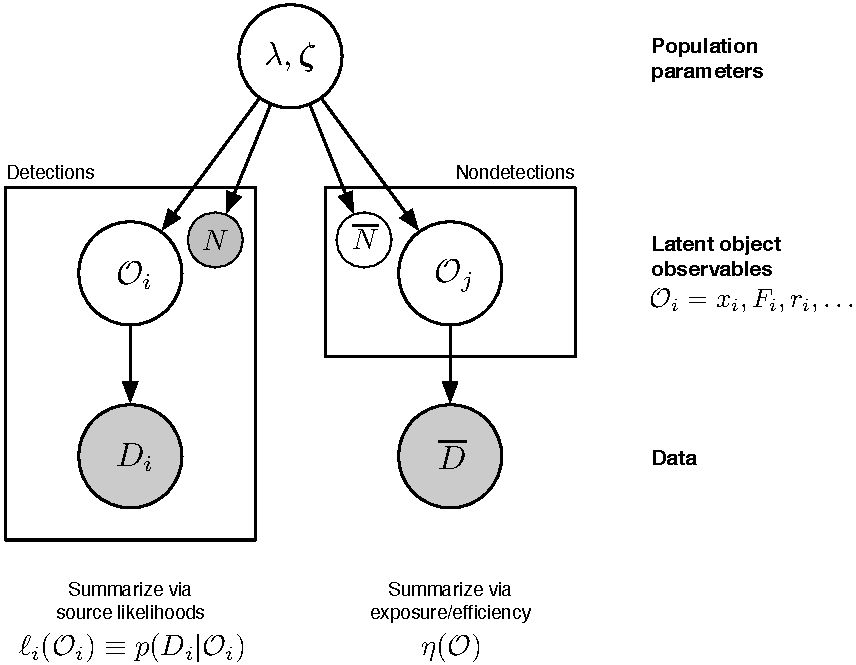
\includegraphics[width=.8\textwidth]{fig/DAG-TLPP}
\end{center}
\caption{Schematic DAG for a thinned latent marked point process model for luminosity function estimation from survey catalog data.
The small $N$ and $\overline{N}$ nodes specify the numbers of replications of the detection and nondetection plates, respectively.}
\label{fig:TLPP}
\end{figure}

Despite these differences with respect to the simpler model structures discussed previously, the structure of the likelihood functions in (\ref{eq:like}) and (\ref{eq:mlike}) is essentially the same as that for conditional density estimation with measurement error (the middle DAG in Fig.~\ref{fig:DAG-TLPP}).
This is because the nondetection part of the DAG in Fig.~\ref{fig:DAG-TLPP} corresponds to a product of exponentials, whose arguments sum in a single integral: the integral on the first line of the likelihood function in (\ref{eq:like}), and in the denominator of the effective densigyt in (\ref{eq:epdf}).
The likelihood or marginal likelihood thus has a single product term, composed of independent factors for each detected object---just the type of structure CUDAHM was designed to sample from.
%\input{TEMP}
%===============================================================================
\section{Luminosity function estimation: Simulation study}
\label{sec:lum_func_sim}

To explore the performance of CUDAHM for luminosity function estimation, we implemented the framework just described and applied it to simulated data.
To focus on performance, this example ignores important complexities arising in modeling real galaxy catalog data.
For example, we ignore cosmological corrections to the inverse square law (which depend on uncertain cosmological parameters).
We also ignore diversity in the spectra of galaxies.
This is important for real data because instruments gather light in limited spectral ranges, determined by properties of the atmosphere, telescope optics, and detector sensitivity.
Among the optical elements are filters that deliberately restrict the spectral passband, so that repeated measurements with different filters can provide broad-band information about galaxy spectra.
As a result, galaxies with the same bolometric (full-spectrum) luminosity and distance, but different spectral shapes, will have different apparent brightnesses (fluxes).
A full analysis would incorporate data from multiple bands.
For the study described here, we assume the simulated galaxies have the same spectra, or that the catalog estimates have been adjusted for spectral diversity.

\subsection{Simulation setup: population parameters and priors}
\label{sec:simsetup-popn}

We simulate observations of a population described by the BB1 model, with parameters chosen so that galaxies with $L>l$ have a distribution similar to that found in the analysis by Blanton et al. (\citealt{blanton2003galaxy}, B03) of $\approx 150,000$ galaxies with spectroscopic redshifts observed in the Sloan Digital Sky Survey (SDSS).
We set $u = 1\times 10^{10} L_\odot$ (where $L_\odot$ denotes the solar luminosity; this is approximately equal to the B03 value of $L_*$ in a Schecter function fit), $\beta = -1.5$ (a bit steeper than the B03 value), and $l= 1\times 10^{8} L_\odot$, corresponding to the lowest luminosities studied by B03.
We choose survey parameters corresponding to a deeper survey than SDSS, thus probing luminosities dimmer than $L=l$.
These choices are motivated in part by current and emerging surveys, such as the photometric (broad-band) surveys by the Panoramic Survey Telescope and Rapid Response System (Pan-STARRS, current) and the Large Synoptic Survey Telescope (LSST; starting in 2023),   and the spectroscopic (redshift) survey by the Dark Energy Spectroscopic Instrument (DESI; starting in 2019).

For distances, we sample values from a spatially homogeneous population extending out to a maximum distance $\rmax = 1$~Gpc.
Only very luminous sources can be detected from large distances.
For the detection criteria we adopt (see below), this maximum distance is such that galaxies are visible beyond $\rmax$ only if $L \gtrsim 20u$, an event with negligible probability (which we formally exclude by truncation).

% suppression factor  $e^{-20} \sim 2\times 10^{-9}$

\enote{Janos also truncated below $l$; is this necessary?}

The upper luminosity scale, $u$, and maximum distance, $\rmax$, together define a fiducial flux value,
\begin{equation}\label{eq:Ffid}
\Ffid
  \equiv \frac{u}{4\pi r_{\rmax}^2} 
  \approx 3.2\times 10^{-13} \left(\frac{u}{10^{10} \Lsol}\right)
      \left(\frac{\rmax}{1~\text{Gpc}}\right)^{-2}\;
      \text{erg cm$^{-2}$ s$^{-1}$}.
\end{equation}
This is a convenient unit in which to express fluxes.
Although $\Ffid$ is minuscule, modern survey telescopes would detect $\sim 10^4$ to $10^5$ photons from a source with this flux.

\enote{Note the parameter value changes!  
The plots need revision; luminosity axis labels need to be shifted by $\times 100$, and the axis label should read $\log_{10}(L/L_\odot)$.  
Check the $\rmax$ value and make sure it corresponds to the flux limit and luminosity truncation after shifting to the new params.}

Now we consider the choice of prior for the population parameters.
For $\beta$, we adopt a prior that is flat with respect to the angle in $\log$-$\log$ space.
This choice has the virtue of not putting a lot of prior probability on the steep slope range, which a flat prior on $\beta$ would do.
Denoting the angle by $\varphi$, if we adopt a prior PDF of $h(\varphi)$ on $\varphi$, the prior on $\beta = \tan\varphi$ is
\begin{equation}
	p(\beta) = \frac{h(\varphi)}{1 + \beta^2}.
\end{equation}
For a flat $\varphi$ prior between two cut-offs $\varphi_L$ and $\varphi_U$,
\begin{equation}
	p(\beta) = \frac{1}{\varphi_U - \varphi_L} \cdot \frac{1}{1 + \beta^2}.
\end{equation}
This is a truncated Cauchy distribution.
The BB2 distribution requires $\beta > -2$, corresponding to $\varphi_L = -1.107$.
If we require Eq.~\ref{eq:lumPDF} to be decreasing, the upper limit becomes $\beta < 0$, corresponding to $\varphi_U = 0$.
Thus, the prior on $\beta$ is
\begin{equation}
p(\beta) = \frac{0.903}{1 + \beta^2} \quad \quad \quad \textrm{for} -2 < \beta < 0.
\end{equation}
For the upper scale we use a log-flat prior, a conventional choice for a scale parameter that must be positive, even though this will be improper on both sides, we can ignore the impropriety and the normalizing constant since the likelihood function will make the posterior proper.
A prior flat in $\log{u}$ corresponds to $p(u) \propto \frac{1}{u}$.
The lower scale $l$ must be below the upper scale $u$, which we can ensure by using a prior factored as $p(l, u) = p(u) p(l \assm u)$ and taking $p(l \assm u)$ to vanish for $l \geq u$.
A log-flat prior also seems appealing for $l$ but the data (i.e. luminosity measurements) do not probe the distribution down to zero due to the flux limit of the telescope, we could not have a proper prior without introduction a lower cut-off.
Instead, we simply use a flat prior on $l$.
Hence, the overall prior will be \begin{equation}\label{eq:popParsPriorPDF} p(\beta, l, u) \propto \frac{l}{u \cdot (1 + \beta^2)} \quad\quad\quad \textrm{for} -2 < \beta < 0, l < u.
\end{equation}

\subsection{Simulation setup: detection and measurement}
\label{sec:simsetup-data}

We simulate measurement errors and selection effects using a simplified model commonly adopted in astronomical simulation studies (\citealt{F99-SDSSSim,LSSTRefDesign}).
Modern astronomical optical detectors, such as cameras using charge-coupled devices (CCDs), count photons.
The Poisson distribution accurately describes photon arrival and detection, but there are additional contributions to measurement uncertainty, including from backgrounds and electronic noise.
To screen out false detections, only reasonably strong candidate sources are accepted as genuine, so that catalog data are typically in the large-counts regime.
Simulation models work in this regime, approximating the Poisson distribution by a normal distribution, and treating the additional contributions to measurement uncertainty also using normal distributions.
The overall measurement uncertainty thus is approximately normal, with a variance found by adding the variances of the component processes.

For simulation studies of hierarchical Bayes approaches, it is important to distinguish approximations of the sampling distribution used to generate simulated data, and approximations of the member likelihood functions needed for inference with a particular simulated dataset.
As a concrete illustration of the distinction, consider a source with true flux $F$ being measured by an idea photon counting detector, with measurement uncertainty due only to Poisson counting uncertainty associated with the source flux.
For an instrument with projected area $A$ observing for a time $T$, the expected number of photons is $\mu = ATF$, and the standard deviation in the number of photons is $\mu^{1/2}$.
In the high-counts regime, we could simulate an observation by drawing a number of photon counts, $n$, from a normal distribution $N(\mu,\mu)$, i.e., with
\begin{equation}\label{eq:PoissonNormal}
p(n|F) \approx \frac{1}{(ATF)^{1/2}\sqrt{2\pi}}
  \exp\left[-\frac{(n-ATF)^2}{2ATF}\right].
\end{equation}
Suppose the simulated value of $n$ is $n_{\rm obs}$.
For analysis of that observation, we would need to approximate the member likelihood function based on that datum.
The exact likelihood function, $\mlike(F)$, based on the Poisson sampling distribution, is proportional to a gamma distribution with shape parameter $\alpha = n_{\rm obs} + 1$ and scale parameter $1/AT$, with its mode at $\hat{F} = n_{\rm obs}/(AT)$, which could serve as a convenient point estimator.
Expressed in terms of $\mu = ATF$, this gamma distribution has mean $\langle ATF\rangle = n_{\rm obs} + 1$ and variance $n_{\rm obs} + 1$.
For large $n_{\rm obs}$, the member likelihood function is thus well approximated by a Gaussian function with mean and variance equal to $n_{\rm obs}+ 1 \approx n_{\rm obs}$:
\begin{align}\label{eq:GammaNormal}
\mlike(F) 
  &\propto \frac{1}{n_{\rm obs}^{1/2}\sqrt{2\pi}}
     \exp\left[-\frac{(ATF - n_{\rm obs})^2}{2n_{\rm obs}}\right]\nonumber\\
  &\propto \exp\left[-\frac{(F - n_{\rm obs}/(AT))^2}
     {2n_{\rm obs}/(AT)^2}\right].
\end{align}
Thus for generating simulated data, we would use a normal distribution, (\ref{eq:PoissonNormal}), with variance depending on the true flux.
But for analyzing a simulated data set, we would use likelihood functions proportional to normal distributions, 
(\ref{eq:PoissonNormal}), with variances depending on the simulated data, $n_{\rm obs}$, for each object.

For our simulations of catalog data, we use normal sampling distributions for estimated fluxes, $\Fhat_i$, with standard deviations that depend on the true fluxes, $F_i$, according to
\begin{align}
\sigma(F)
  &= \sqrt{\sigma_0^2+(\alpha F)^2}\nonumber\\
  &= \sigma_0 \left[1 + \left(\frac{\alpha F}{\sigma_0}\right)^2 \right]^{1/2},
\label{eq:sig-F}
\end{align}
where $\sigma_0$ characterizes the noise contributions from backgrounds and detector electronics, and $\alpha$ characterizes how Poisson fluctuations in the number of detected photons influence $\Fhat_i$, relative to the flux-independent noise sources.
For an object with simulated best-fit flux $\Fhat_i$, we use a member likelihood function that is a Gaussian function with mode at $\Fhat_i$ and standard deviation parameter
\begin{equation}
\hat{\sigma}_i(\Fhat)
  = \sqrt{\sigma_0^2+(\alpha \Fhat_i)^2},
\label{eq:sig-Fhat}
\end{equation}
using the same values for $\sigma_0$ and $\alpha$ as are used for the sampling distributions.
Based on published simulations of existing and anticipated surveys (\citealt{F99-SDSSSim,LSSTRefDesign}), we set $\alpha = 10^{-2}$ for our simulations.
We set $\sigma_0 = 6.4\times 10^{-10}$ and $\alpha = 10^{-2}$ and $\sigma_0 = 6.4\times 10^{-10}$~erg~cm$^{-2}$~s$^{-1}$ for our simulations.
The latter value was chosen so that sources with $L=20 u$ at $r=\rmax$ are just detectable by the error-based detection criterion described below.


\enote{Check these error/threshold params; they should correspond to Janos's values shifted to physical units.}

For detection, we require a candidate object to have estimated flux a factor $\nu = 5$ times the measurement error.
This corresponds to a threshold flux satisfying $\Fth = \nu \hat{\sigma}_i(\Fth)$, which gives
\begin{equation}\label{eq:Fth}
\Fth = \frac{\nu \sigma_0}{\sqrt{1-\alpha^2}}.
\end{equation}
For the parameters of our simulation, this corresponds to $\Fth = X$.
The detection efficiency is the probability that the measured value, $\Fth$, for a source with true flux $F$ will be above the threshold,
\begin{align}\label{key}
\eta(F)
  &= p(\Fhat > \Fth|F)\nonumber\\
  &= \Phi\left(\frac{F - \Fth}{\sigma(F)}\right),
\end{align}
where $\Phi(\cdot)$ denotes the standard normal cumulative distribution function.



%-------------------------------------------------------------------------------
\subsection{Simulation setup}
\label{sec:simsetup}


\enote{IGNORE THIS SUBSECTION.}


In case of real measurements the distance of the objects is known from redshift observations.
In our simplified case we assume these distance measurements to be without error.
To compile the simulated data set, we assume a spherically symmetric, homogeneous distribution of galaxies and generate the random distances $r_i$ accordingly.
We use the inverse-square law
\begin{equation}
F_i = \frac{L_i}{4 \pi r_i^2}.
\end{equation}
The observational noise $E$ of the flux $F$ is modeled as Gaussian with zero mean and a standard deviation of
\begin{equation}
\sigma(F)=\sqrt{\sigma_0^2+(0.01F)^2}.
\label{eq:error}
\end{equation}
The flux limit of the telescope is the constant $T$ and $C$ will denote the event when an object is detected, i.e. the noisy flux is above the threshold: $D > T$.
When generating the random sample, the luminosity is limited between $10 \leq \log_{10}{L} \leq 14$ which implies the distance limit
\begin{equation}
r_\textnormal{max} = \sqrt{\frac{L_\textnormal{max}}{4 \pi T}}.
\end{equation}

As it was discussed above in Sec.~\ref{sec:intro}, the spatial distribution of galaxies is considered homogeneous, hence the density function becomes \begin{equation}\label{eq:dist_dens_func}
\delta(r) = 
\begin{cases} 
    \dfrac{3r^{2}}{r_{\max}^{3}} & \quad \text{if } 0\leq r\leq r_{\max}\\
    0 & \quad \text{otherwise}
\end{cases} 
\end{equation}
and the cumulative distribution function: \begin{align}\label{eq:dist_cum_func} \Delta(r)= \begin{cases} 0 & \quad \text{if } r<0\\ \dfrac{r^{3}}{r_{\max}^{3}} & \quad \text{if } 0\leq r\leq r_{\max}\\ 1 & \quad \text{if } r\geq r_{\max} \end{cases} \end{align}


To take the selection effect of the flux limit into account, we have to calculate the probability of measuring a galaxy with a given luminosity and distance above the flux limit.
By assuming Gaussian noise, as we already did in Sec.~\ref{sec:bb1truncpl}, the sought probability becomes
\begin{align}
p(C | L, r) &= p(C | F) = \Pr(D>T | F)\\
&= \Pr(F+E>T)\\
&=\Pr(\underbrace{F + E}_\text{$\sim \mathcal{N}\left(F,\sigma(F)\right)$} > T)\\
&=\frac{1}{2}\left( 1 + \erf\left( \frac{F - T}{\sqrt{2}\sigma(F)} \right) \right)\\
&=:\zeta(F ; T,\sigma_0)
\label{eq:pclr}
\end{align}



%-------------------------------------------------------------------------------
\subsection{Case study}

\enote{Tables and plots need to be adjusted here to shift to new units.}

We apply the hierarchical Bayesian model to estimate the model parameters of a simulated random sample of $100{,}000$ galaxies.
We compare the results of the Bayesian analysis to maximum likelihood and evaluate the performance of the GPU-based implementation.
The true values of the population parameters are listed in the first row of Tab.~\ref{tab:sum_est}.
The value of $\sigma_0$ in Eq.~\ref{eq:error} is chosen to be $\sigma_0=1$.
The flux limit is $T = 5.0$ and the distance limit is $r_{\max} \gtrsim 1.12 \times 10^{6}$.

We executed 1.5M burn-in and the same number of live MCMC steps to sample the probability distribution of the population parameters.
The length of the burn-in sequence was chosen by visual inspection of the autocorrelation plots.
To reduce autocorrelations in the Markov chain, $\theta$ samples were thinned and only every $150^\textnormal{th}$ sample was kept, hence the final number of samples was $10{,}000$.
Fig.~\ref{fig:results} shows the traces, histograms and autocorrelation plots of the population parameters whereas Tab.~\ref{tab:sum_est} lists the result in a numerical format.

\begin{table} \begin{center} \begin{tabular}{ l | d{12} | d{12} | d{12} | } \cline{2-4} & \beta & l & u \\ \hline \multicolumn{1}{|l|}{$\theta_\text{true}$} & -1.5 & 5.0\hphantom{000} \times 10^{10} & 5.0\hphantom{000} \times 10^{12} \\ \hline \multicolumn{1}{|l|}{$\theta_{\text{MCMC}}$} & -1.5037 & 5.0302 \times 10^{10} & 5.0000 \times 10^{12} \\ \hline \multicolumn{1}{|l|}{$\sigma_{\theta\text{,MCMC}}$} & 0.0059 & 3.3548 \times 10^{9} & 3.1806 \times 10^{10} \\ \hline \multicolumn{1}{|l|}{$\theta_{\text{MLE}}$} & -1.5564 & 7.3222 \times 10^{10} & 5.7207 \times 10^{12} \\ \hline \multicolumn{1}{|l|}{$\theta_{\text{MLE, no noise}}$} & -1.5009 & 4.9341 \times 10^{10} & 4.9819 \times 10^{12} \\ \hline \multicolumn{1}{|l|}{$\lvert \theta_{\text{true}} - \theta_{\text{MLE}} \rvert$} & >9.5525 \cdot \sigma_{\beta\text{,MCMC}} & >6.9221\cdot\sigma_{l\text{,MCMC}} & >22.6591\cdot\sigma_{u\text{,MCMC}} \\ \hline \end{tabular} \end{center} \caption{Summary of parameter estimation results.
The first row of the table indicates the true values which the simulated data was generated with.
The second row shows the mean of the distributions coming of the Bayesian model, whereas the third row contains the standard deviation of them.
For reference, we indicate the outcome of the ML estimatior run on the simulated data with and without noise in rows 4~and~5, respectively.
To compare the Bayesian model to ML, the last row of the table shows the difference between the ML estimator and the true values in terms of the standard deviation of the posterior from the Bayesian model.} \label{tab:sum_est} \end{table}

\begin{figure}
    \centering
    \begin{subfigure}{0.3\textwidth}
        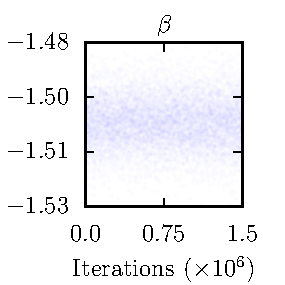
\includegraphics{{fig/beta}}
    \end{subfigure}
    \begin{subfigure}{0.3\textwidth}
        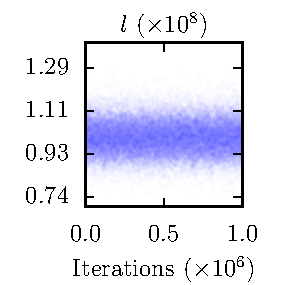
\includegraphics{{fig/lowerscale}}
    \end{subfigure}
    \begin{subfigure}{0.3\textwidth}
        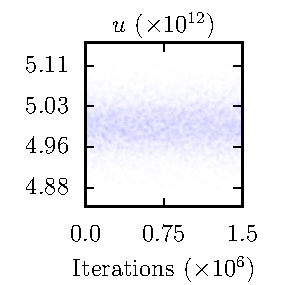
\includegraphics{{fig/upperscale}}
    \end{subfigure}
    
    \begin{subfigure}{0.3\textwidth}
        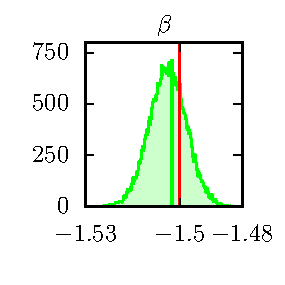
\includegraphics{{fig/beta_histo}}
    \end{subfigure}
    \begin{subfigure}{0.3\textwidth}
        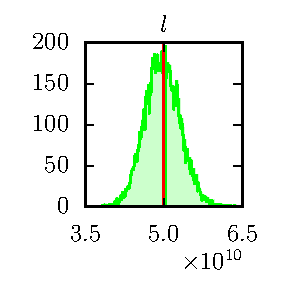
\includegraphics{{fig/lowerscale_histo}}
    \end{subfigure}
    \begin{subfigure}{0.3\textwidth}
        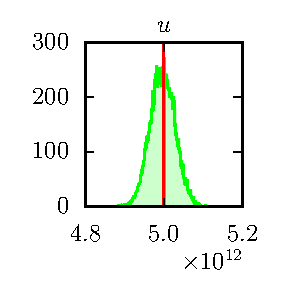
\includegraphics{{fig/upperscale_histo}}
    \end{subfigure}    
    
    \begin{subfigure}{0.3\textwidth}
        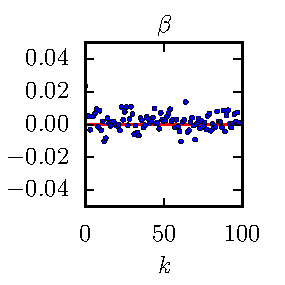
\includegraphics{{fig/autocorr_beta}}
    \end{subfigure}
    \begin{subfigure}{0.3\textwidth}
        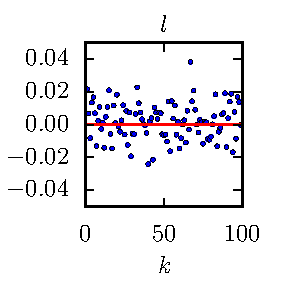
\includegraphics{{fig/autocorr_lowerscale}}
    \end{subfigure}
    \begin{subfigure}{0.3\textwidth}
        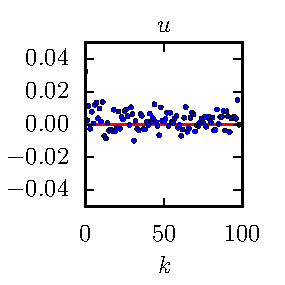
\includegraphics{{fig/autocorr_upperscale}}
    \end{subfigure}    
    \caption{Trace (upper row), histogram (middle row) and autocorrelation (lower row) plots of the three population parameters. The red vertical line overplotted the histograms show the true value of the parameter. With the exception of $\beta$, Bayesian modelling can recover model parameters with excellent accuracy.}
	\label{fig:results}
\end{figure}

%-------------------------------------------------------------------------------
\subsection{Performance tests}

\begin{figure}
   	\begin{center}
   		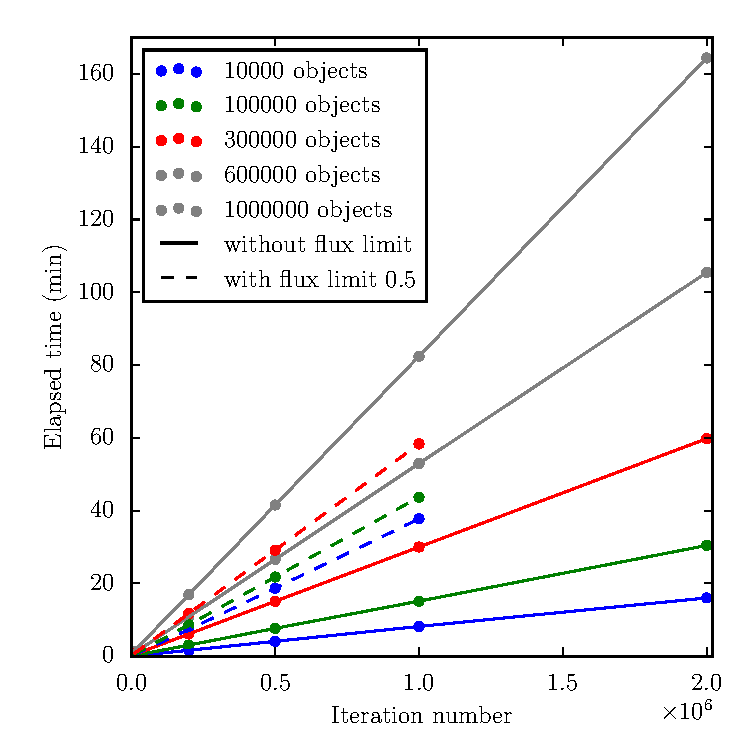
\includegraphics{{fig/performance_iter_vs_time}}
   	\end{center} 
    \caption{Runtime of the GPU code as a function of iterations for different numbers of objects, with (solid lines) and without (dashed lines) considering a flux limit of $T = 0.5$. Taking the flux limit into account results in an approximately fourfold increase of runtime.}
    \label{fig:performance_iter_vs_time}
\end{figure}

\begin{figure}
   	\begin{center}
   		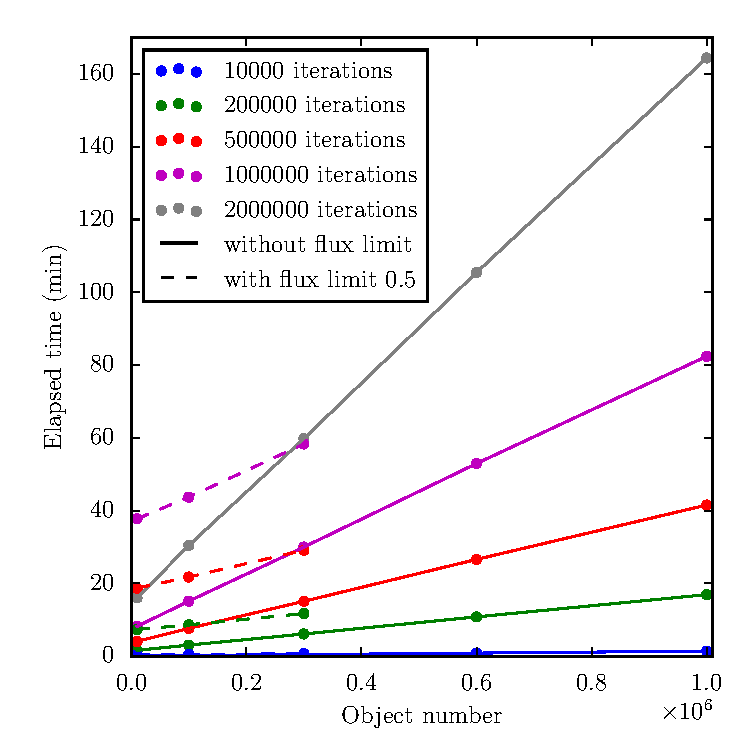
\includegraphics{{fig/performance_obj_vs_time}}
   	\end{center} 
    \caption{Runtime of the GPU code as a function of the number of objects, after a given number of iterations, with (solid lines) and without (dashed lines) considering a flux limit of $T = 0.5$. Taking the flux limit into account results in an approximately fourfold increase of runtime. On the other hand, the scaling of runtime with the number of objects is linear. This is due to the fact that fluxes are statistical independence, hence their distribution can be sampled in parallel on the GPU.}
    \label{fig:performance_obj_vs_time}
\end{figure}

We used NVIDIA Tesla K40c cards for the performance tests.
First, we executed tests without imposing a flux limit, which is a much simpler case as it does not contain the time-consuming numerical integration of Eq.~\ref{eq:mu}.
Next, we executed the with the flux limit turned on.
Fig.~\ref{fig:performance_iter_vs_time} shows the elapsed time as a function of iteration number (non-thinned) for different number of objects.
The functions are trivially linear as iteration steps always take a fixed amount of time.
More informative is Fig.~\ref{fig:performance_obj_vs_time} where we plot the elapsed time as a function of the number of objects for various numbers of iteration steps.
The linear scaling of computation time with the number of objects is due to the fact that the characteristics are independent.
As it is visible from the figures, turning on the flux limit clearly decreases the performance.
Real galaxy catalogs contain objects on the order of $10^8$, two magnitudes more than our simulated data set.
Extrapolating from out performance numbers, estimating the parameters of the luminosity function with $2 \times 10^5$ Markov steps would take about 2000 minutes, a bit less then one and a half days, which makes applying our method to real data feasible.



%===============================================================================
\section{Summary}
\label{sec:summary}

We have described a usefully general \Cpp\ framework for massively parallel implementation of simple hierarchical Bayesian models.
We have applied this framework to estimating luminosity functions of objects measured with uncertainty, and subject to (quantified) selection effects.
Our implementation shows linear scaling with both, the number of Markov chain iterations and the number of objects, which makes it applicable to real data sets of size up to $10^{8}$ using modest-sized clusters of GPUs.



\section*{Acknowledgments}

The CUDAHM project began in a working group affiliated with the Program on Statistical and Computational Methodology for Massive Datasets hosted by the Statistical and Applied Mathematical Sciences Institute (SAMSI) in 2012--2013.
This paper was completed as part of the 2016--2017 SAMSI Program on Statistical, Mathematical and Computational Methods for Astronomy.
Budav\'ari, Kelly, and Loredo are grateful to SAMSI for support of this work.
Loredo's work on this project was also supported by NSF grant AST-1312903.
Szalai-Gindl's work was supported by the Hungarian Scientific Research Fund via grant OTKA~NN~114560.


% \bigskip \begin{center} {\large\bf SUPPLEMENTARY MATERIAL} \end{center}

\section{Computing $\mu(\theta)$}
\label{sec:comp_mu_theta}


We want to compute the following integral numerically:
\begin{equation}
\mu(\theta) = \int_{0}^{\infty} \dd r \int_{0}^{\infty} \dd L \; \zeta\left(\frac{L}{4\pi r^2},T,\sigma_{0}\right)\cdot\lfunc(L|\theta)\cdot \delta(r),
\label{eq:mu_mu}
\end{equation}
where
\begin{equation}
\zeta(F ; T,\sigma_{0}) =
	\frac{1}{2}\left( 1 + \erf\left( \frac{F - T}{\sqrt{2} \cdot \sqrt{\sigma_{0}^2+(0.01 F)^2}} \right) \right).
	\label{eq:mu_zeta}
\end{equation}
It turns out that direct numerical integration of Eq.~\ref{eq:mu_mu} using the \texttt{cubature} package \citep{johnsoncubature} is unstable due to the very steep nature of the error function part.
We plot the argument of the error function $A = \frac{F - T}{\sqrt{2\cdot(\sigma_{0}^2 + (0.01 F)^2)}}$ in Fig.~\ref{fig:erfArg} as a function of $F$ for reference.
The value of $A$ approaches $\frac{1}{\sqrt{2}\cdot 0.01} \approx 70.710678 $ in the $F \rightarrow \infty$ limit.
For any value $c < \frac{1}{\sqrt{2}\cdot 0.01}$, the inverse error function yields $X = \erf^{-1}{c} = \frac{T+\sqrt{2}c\cdot \sqrt{(1-2(0.01)^2 c^2)\sigma_{0}^2 + (0.01)^2 T^2}}{1-2(0.01)^2 c^2}$.
In luminosity units, $X$ corresponds to $L = 4\pi r^2_\textrm{max}X$.
We can approximate the error function by $1$ if its argument is sufficiently large.
For our purposes $c > 6$ is a good choice (the equivalent of a $6\sigma$ measurement error), for which $\erf(6.0) \approx 0.9999999999999999784803$.
Hence, we split the integral in Eq.~\ref{eq:mu_mu} into two intervals: $F < X$ and $X \leq F$, corresponding to $L < 4\pi r^2 X$ and $L \leq 4\pi r^2 X$.
To avoid the variable $r$ in the limit of the integration, we will use the constant $ 4\pi r^2_\textrm{max} X$ as the threshold.
Eq.~\ref{eq:mu_mu} becomes 
\begin{align}
\label{eq:mu_approx}
\mu(\theta)
  &=\int_{0}^{r_{max}} \int_{0}^{\infty} \zeta\left(\frac{L}{4\pi r^2} ; T,\sigma_{0}\right)\cdot\lfunc(L ; \theta)\cdot \delta(r)\, \dd L \, \dd r\\
  &\approx \int_{0}^{r_{max}} \int_{0}^{4\pi r_{\max}^2 X} \zeta\left(\frac{L}{4\pi r^2} ; T,\sigma_{0}\right)\cdot\lfunc(L ; \theta)\cdot \delta(r)\, \dd L \, \dd r\\
  &\qquad + \int_{0}^{r_{max}} \delta(r)\cdot\int_{4\pi r_{\max}^2 X}^{\infty} \lfunc(L ; \theta)\, \dd L \, \dd r\\
  &= \int_{0}^{r_{max}} \int_{0}^{4\pi r_{\max}^2 X} \zeta\left(\frac{L}{4\pi r^2} ; T,\sigma_{0}\right)\cdot\lfunc(L ; \theta)\cdot \delta(r)\, \dd L \, \dd r\\
  &\qquad + 1 - \clfunc(4\pi r_{\max}^2 X ; \theta),
\end{align}
where we made the approximation $\zeta(F ; T,\sigma_{0}) \approx 1$ for $X \leq F$.
The numerical integral of the first term now converges and we can integrate the second term by parts analytically.
One can recognize Eq.~\ref{eq:lumCDF}, the cumulative probability function of luminosity in the result, which can be computed directly.

\begin{figure}
\begin{center}
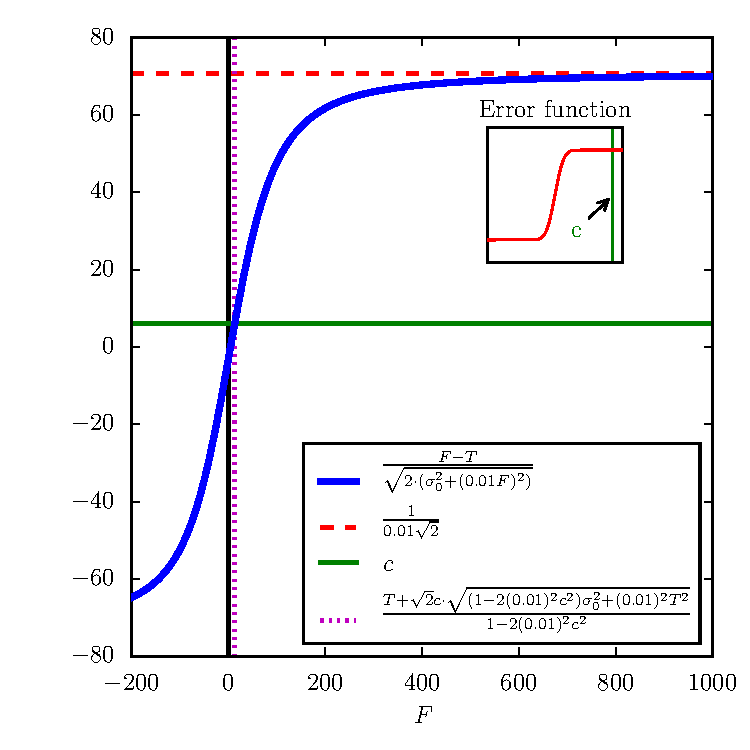
\includegraphics{{fig/erfArg}}
\end{center}
\caption{The argument of the error function in Eq.~\ref{eq:mu_zeta} (blue curve). See text for discussion.}
\label{fig:erfArg}
\end{figure}


\bibliographystyle{agsm}

\bibliography{CUDAHM}

\end{document}
